%%%%%%%%%%%%%%%%%%%%%%%%%%%%%%%%%
% 6CCS3PRJ Final Year Individual Project Report
% luke.day@kcl.ac.uk
%%%%%%%%%%%%%%%%%%%%%%%%%%%%%%%%%
\documentclass[11pt]{informatics-report}
\usepackage{color}
\usepackage[square,sort,comma,numbers]{natbib} %References

%%%%%%%%%%%%%%%%%%%%%%%%%%%%%%%%%
% Front Matter - project title, name, supervisor name and date
%%%%%%%%%%%%%%%%%%%%%%%%%%%%%%%%%
\title{7CCS3PRJ Final Year\\\vspace{0.2cm}Individual Project Report Title}
\author{Maciej Musialek}
\studentID{K1208837}
\supervisor{Elizabeth Black & Elizabeth Sklar}

\date{\today}

\abstractFile{FrontMatter/abstract.tex}
\ackFile{FrontMatter/acknowledgements.tex} %Remove line if you do not want acknowledgements

\begin{document}
\createFrontMatter
\onehalfspacing
\tableofcontents
\doublespacing

%%%%%%%%%%%%%%%%%%%%%%%%%%%%%%%%%
% Report Content
%%%%%%%%%%%%%%%%%%%%%%%%%%%%%%%%%
% You can write each chapter directly here or in a separate .tex file and use the include command.

\chapter{Introduction}
This is one of the most important components of the report. It should begin with a clear statement of what the project is about so that the nature and scope of the project can be understood by a lay reader. It should summarise everything that you set out to achieve, provide a clear summary of the project's background and relevance to other work, and give pointers to the remaining sections of the report, which will contain the bulk of the technical material.

\section{Report Structure}

\chapter{Background}
Before setting off to outline what has been finished in the project and how certain choices were made in comparison to others, the report will be discussing the current situation of the robotics community and the human-robot collaboration in general for how the robots communicate with each other. Also a more detailed outline onto the treasure hunt game will be given to give a better image of why this research was chosen over others.

    With this in mind, it is important to outline what ideas are currently looked at and how they influence the field of robotics and more importantly, what they bring to the project. In the following sections, an outline of the treasure hunt game along with two main areas of research in robotics that are relevant to this report will be given. These evaluations will be concerning human-robot collaboration and research that was focused around the ROS environment.

    \section{Treasure Hunt Game}
      Following the introduction that said that this report will focus on creating a treasure hunt game, it is important to understand the concepts behind the game. The games aim is not to create a competitive game where users will interact. The main goal is to test the communication between various robots. With that said the following explanation will give an outline to how the game works and this explanation is directly inspired by Sklar and Azhar’s paper on ArgumentationBased Dialogue Games for Shared Control in Human-Robot Systems.

      The game works by using a simulation environment between a robot and a human. In this environment there is a map with hidden treasures, a robot that explores it as well as a human suggesting where the robot should go. The person that controls the robot gives commands as to which room the robot should visit first along with an option to ask the robot for its opinion on the matter. This gives room to possibilities of dialogue communication between two parties and as such give a robot the chance to persuade the user towards a better option.

      There are numerous possibilities for the treasures and their identification is important to yield different results as well as to use as little energy as possible to get a maximum score. This score can then be evaluated to see how the robot influenced the user and how the communication influenced the experience for the human as well as the score. This then can be used to decide the best strategy for dialogues. The possibilities for treasures can be demonstrated by a figure taken from Sklar and Azhar’s paper[1] which can be found below for ease of access.

        \begin{figure}[!ht]
          
          \centering
            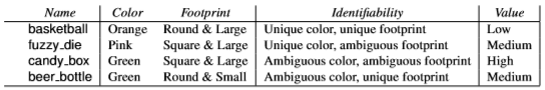
\includegraphics[width=1.02\textwidth]{figures/treasures.png}
            \caption{Example of Treasures in the game.}
        \end{figure}

      With these treasures it is easy to see how users might make errors between treasures that carry high ambiguity but also shows how it is unnecessary to use up energy for taking pictures of treasures that have very unique qualities and with that, can be simply grabbed for increasing the score. This could be developed in the environment to ensure that the robot makes sure that the user is certain of taking pictures of treasures that are implicitly unique.

      The game also makes the robot energy a precious resource with robot losing energy for practically every action that it takes apart from communicating with the user.

      This leads to the motivation in this report of creating this environment with customizability of Dialogues as well as ensuring that a multi robot environment is allowed to further see how increasing the number of robots affect the dialogue experience in Human-Robot communication.

    \section{Related work in Human-Robot collaboration}
      Currently research is greatly focused on human-robot collaboration for humans and robots in the same environment, working simultaneously on a task together. This in turn makes the current problem more unique. The problem we consider in this paper works on the assumption that humans and robots are in separate environments, and with that the robot can potentially have a lot of control over the environment. The following subsections give a more precise background in research of human-robot collaboration.

      \subsubsection{Same space collaboration}
        In their papers Liu et al.\cite{ChangLiu} and Govindarajan et al.\cite{Vijay} discuss collaboration in same space. 

        In the first paper\cite{ChangLiu} the collaboration is outlined by robot working together with the human. The setup of the experiment was to give each human-robot team a group of tasks that either required one agent to complete or a joint task for both of them. The aim was to finish a list of tasks as quickly as possible. The measurement parameters were mainly the fluency of collaboration outlined by Hoffman's metrics. Their results found many conclusions; one of which was that humans preferred working with robots that could infer plans based on human movement. This gives an implication to the project that ultimately guides the project to try and develop a robot that could propose movements as to giving the human full power over the environment and the process. In that way it can be considered good practice to let an idle robot move based on its own path planner to the closest room if it was neglected. This of course, is subject to human preference but allowing such functionality could be considered.

        In Govindarajan et al's\cite{Vijay} paper the main focus of research was search and rescue actions where robots infer different paths from where the human is headed thus maximizing the search space of a room. To develop an algorithm that would handle the robots, the researchers used the ROS platform. In their results they have found that using complementary homotopy classes for intelligent path finding increased the performance of robots helping them make more intelligent decisions. While not particularly useful for robots that search different rooms, using homotopy classes for finding out which robot should potentially reach specific rooms could be useful when making plans that revolve around finding maximum number of rooms helping robots achieve more efficient paths. Additionally another area of research would be with large amount of robots. In that research the robots would use homotopy classes to make decisions based on first movements of robots to try and predict which would be the next rooms that the current robot would choose. With that, the robots would move away from that area that will potentially be visited anyway to start exploring other areas.

      \subsubsection{Spatial recognition}
        Goto et al.'s\cite{Hiraki} paper work on maximizing fluency in human-robot collaboration and identifying challenges posed by robots when it comes to recognizing parts that would be required for assembly of parts. To achieve this they focused on a finite state machine approach for robots to help with table assembly. This can be considered a more limited approach in terms of robot intelligence since robots are limited in the amount of states they will be in. In their results they managed to see limitations with the robot both recognizing the human action and with the scalability of the software due to most of it being hand made beforehand. The paper mainly focused on being able to achieve the task in comparison to achieving the task efficiently or effectively. With that in mind it poses considerations that need to be taken when looking at robot design one of the most important being a challenge being the robot understanding what it sees and how limited they can be when it comes to object recognition.

      \subsubsection{Modalities of human preference}
        While in their paper Fiore et al.\cite{Fiore} did not use the robot operating system, they embarked on a task that would prove that robots are capable of completing collaborative tasks based on human supervision. In this sense, their paper is very related to research outlined in this paper. Fiore et al. Propose a complex system that is built on sophisticated software for intention inference, path planning, task execution and communication. In their results they have proved that the system is capable of: handling joint goals and actions, handling users preferences, handling agent beliefs and monitoring human actions. With that in mind, a multitude of research has been proposed in creating human-robot collaboration and proving that the tasks are in fact possible complete.

      \subsubsection{Conclusion}
        It seems that a lot of current research has put a great focus on proving that human robot collaboration is indeed possible with a huge variation of approaches between each paper. While quite a new area, it is important to note that currently, there doesn't seem to be a greater standard in how research is carried out with researchers assembling software based on their research preference. It does not dispute the fact that every research paper proposes new considerations in human-robot collaboration and that possible improvements are drawn based on their approaches.

        This leads to a conclusion that Human-Robot collaboration is a very undeveloped field and will start presenting more exciting opportunities in the future for researchers to look at. Currently it seems that a great deal of effort is in ensuring that fluency between agents is maximized making the experience faster and more enjoyable for the participant in the study and potential agents for developed systems in the future.
    
    \section{Research in ROS environment}
        The reason for choosing to research ROS in greater detail is that it will be the main platform that runs the robotics simulations in this Project. In essence, it will be the backbone of the system and a lot of work will be determined by the success of its implementation. To achieve this, a solid background on how it was used in the past and what it has been used for is considered to ensure that the wheel has not been reinvented as well as to see potential uses of ROS to later on expand the system when it is developed.

        In comparison to previous research that focused on proving various possibilities of robotics systems, research that focuses on using ROS environment is mostly aimed towards developing various frameworks to ease the use of the environment to achieve certain results. As such, it can be compared to human-robot collaboration research as focusing more on solving problems than proving. Following sections outline various works that used the ROS environment to achieve their goals.

      \subsubsection{Frameworks}
        In their two papers Fok et al.\cite{ChienLiang} and Liang S Ng et al.\cite{Liang} focus on creating two separate networks that provide an interface for grabbing robots and control for complex whole body robots with multiple parts. In both of the papers, ROS was being used which stands to justify just how powerful ROS can be in manipulating various environments. In fact, the paper on creating a hardware and software problem for intelligent applications, is very similar to the approach this report is focused on. The simulation platform is in fact exact with the only difference being controlling single robots forwards and backwards rather than using path planning for the problem. From these findings, given time, the report can be further studied to include complex body robots that can be controlled over the cloud with hand held devices. This only signifies the availability of technology for implementing complex robot systems using ROS.

      \subsubsection{Domain specific research}
        Deusdado et al.'s\cite{Pedro} research focused on creating an aerial-ground teams in ROS for systematic soil and biota in estaurine sampling. Mario Vieira et al.'s research further focused on creating applications for monitoring human daily activity and risk situations in robot-assisted living. Both of these papers can be considered extremely centered around the areas that they focus on and show the variety of scenarios that ROS can be used for. Both teams achieved great success in their plan to centralize use of ROS for their respective goals and showed how useful they can be in further research. The first paper gives us an idea of how ROS can be used to implement robot teams, giving us ideas about how to space out cloud platforms to further enrich the environment while the second, allows us to see how to use robot sensors to view activity of humans. 

        This knowledge, can in fact be extrapolated to the project in future works to give a richer environment. One where each robot is directly responsive to actions of the other through the use of sensors rather than shared goal reaching creating a more human like collaboration not only between the robot and the human but throughout the whole team. It is important to note that while right now the robots focus is to reach desired destinations and share data to produce better maps. An alternative of proposed research above shows us that using a more intuitive approach can be just as useful.

      \subsubsection{Conclusion on ROS research}
        It is very easy to see that ROS research and implementations revolves around creating better frameworks and centralized domain problem solving. It is a very young field that so far didn't set standards towards what would be the best approach so that researchers could start tackling these issues and start improving on standard solutions. This in turn, emphasizes that the field is going to expand creating more elaborate solutions and frameworks for specific domain problems. At the time this report was written, most papers presented here are papers that came out in 2016th to ensure that the image of current affairs is as accurate as possible. With this information, as presented above ideas can be drawn about possible improvements to the implementation that could in turn create an environment where the collaboration is as fluent as possible with robots taking same type of initiative that normal humans would.

      \section{ROS challenges posed by its creators and community}
        Currently ROS is an overwhelmingly expanding software with new additions being added. ROS started in 2010 and already had 9 releases with the 10th coming out in May 2016. This sort of expansion rate pushes developers to re-learn the structure and standards set by ROS every few months, in turn making the frameworks obsolete every 8 months or so IF they used code that ROS creators deemed unnecessary in future releases or made it deprecated through certain decisions. This challenge is actually an obstacle for ROS creators themselves as in some examples, the Wiki pages can reference functions that can be considered deprecated in future releases. This in turn makes developers turn to the ROS community which is limited to the small group of robotics specialists using ROS that are willing to help on answers.ros.org.

        The community itself is compromised of a fairly small amount of user group that cannot be compared to regular software developer websites like StackOverflow or BigResource where commercial development and advice seeking can start to compare itself to a competition of its own. This produces problems when a regular developer that didn't have much experience with the environment, thus making it harder to develop in this network.

        It is also extremely important to note that at this point in time there is a huge deficit in the amount of available resources the developer can reference to when it comes their struggles. The few books that do exist to help users develop their knowledge are few and their knowledge as previously stated can become obsolete extremely fast due to ROS's quick expansion rate. When this report was created, there were also no current frameworks available for faster safer development or third party libraries to help a developer create a bigger understanding which means that the wheel of development for ROS is mostly reinvented every time a new idea is presented for development. This leads to a conclusion that the outlined specification will be extremely challenging posing a lot of stalls for implementation of the software.
        
    \section{Conclusion}
      It is clear that ROS is an amazing platform offering its users a great diversity in use. The research in human-robot collaboration and ROS is starting to expand the use of ROS in human-robot collaboration is starting to slowly become a standard. This in turn means, that selecting ROS as a developer platform for robot simulation is definitely a right fit for this project.

      With the previous section, it is clear that there will be challenges in this project that might in fact not get fulfilled simply due to lack of resources that will be able to acquire and through that, a careful consideration will be taken to ensure that the goals are realistic and not reaching outside the scope of the possibilities.
\chapter{Report Body}
The central part of the report usually consists of three or four chapters detailing the technical work undertaken during the project. {\bf{\textcolor{red}{The structure of these chapters is highly project dependent}}}. They can reflect the chronological development of the project, e.g. design, implementation, experimentation, optimisation, evaluation, etc (although this is not always the best approach). However you choose to structure this part of the report, you should make it clear how you arrived at your chosen approach in preference to other alternatives. In terms of the software that you produce, you should describe and justify the design of your programs at some high level, e.g. using OMT, Z, VDL, etc., and you should document any interesting problems with, or features of, your implementation. Integration and testing are also important to discuss in some cases. You may include fragments of your source code in the main body of the report to illustrate points; the full source code is included in an appendix to your written report.

\section{Section Heading}

\subsection{Subsection Heading}
\chapter{Specification for the report}
    To ensure a good outline of the project is given specification needs to be provided for various parts of the system to later on lead the design, implementation and testing of the environment. The following sections break down the system into its biggest parts and give a set of requirements as guidelines.

    \section{The simulation environment}
      The robot environment will be the center of emulating the environment. It will be responsible for housing the Robot Operating System server with maps, odometry for robots and mapping the robots inside a map so that they will be able to move around and accept commands from outside sources i.e. the GUI and transfer these commands into robot movement and task allocation. Below is the outlined specification for the environment.

      \begin{itemize}
        \item \textbf{SE1}: ROS based simulation environment.
        \item \textbf{SE2}: An environment that allows simulation of a robot on a 2-D plane with the map received from project supervisor.
        \item \textbf{SE3}: Accepting commands from outside sources that guide the robot e.g. Go to room 1.
        \item \textbf{SE4}: Responding to commands about robots position and whether it reached its goal.
        \item \textbf{SE5}: An ability for the robot to realize which rooms are closest to it.
        \item \textbf{SE6}: Robot is able to find its own way inside the map to the goal.
        \item \textbf{SE7}: Allow for more than one robot in a single simulation.
        \item \textbf{SE8}: Robot is fully aware of another robots presence.
        \item \textbf{SE9}: Robot is able to avoid collisions with other robots.
        \item \textbf{SE10}: The environment can accept various maps and robots can adapt to these.
        \item \textbf{SE11}:  (Optional) Simulation minimizes the use of system resources.
      \end{itemize}

    \section{Graphical User Interface}
      The Graphical User Interface is a crucial aspect to how the task distribution will be managed. Whether it is click and go or hot keyed commands is a question that will be crucial here. The human factor needs to be taken into account as basis for testing but having a user interface that doesn't allow comfortable work will only result in slowing down the human factor and making the results biased towards the robots working by themselves. Below is the outlined specification for the GUI.
      
        \begin{itemize}
          \item \textbf{UI1}: Interface should provide an approximated view of the simulation.
          \item \textbf{UI2}: Interface provides options for users to select rooms that robots go to.
          \item \textbf{UI3}: Users are able to select robots that they want to send goals for.
          \item \textbf{UI4}: User has the option of identifying the treasure, taking the picture and moving on.
          \item \textbf{UI5}: Upon receiving the picture user has the option to take the treasure.
          \item \textbf{UI6}: Interface contains the map with an outline of rooms.
          \item \textbf{UI7}: Interface updates robots positions on the map based on where they are in the simulation.
          \item \textbf{UI8}: Interface accepts various Dialogues when a command is executed to show to the user.
          \item \textbf{UI9}: (Optional) Keyboard shortcuts implemented to smooth out the job as opposed to point and click where a mouse has to move all the time.
        \end{itemize}
    \section{Dialogue Interface}
      Testing the environment that was developed to the specification is the main focus of this project. It is however important to ensure that various models of communication are allowed to be ran to make the system usable and fulfill its purpose as research assistance and possibly assistance in the future for developing systems. Below are some main requirements for the dialogue interface.

        \begin{itemize}
          \item \textbf{DI1}: Hold necessary dialogues for different scenarios(Select room, Take a picture, Take treasure)
          \item \textbf{DI2}: Cater to different amounts of responses.
          \item \textbf{DI3}: Be outside of the GUI to ensure modularity.
          \item \textbf{DI4}: (Optional) Allow an array of responses for a given action(Two different sentences for the same action).
          \item \textbf{DI5}: Dialogue possibilities held on an external file.
        \end{itemize}

  \chapter{Design}

    The systems goal is to simulate a robot environment with multiple possible robots on the platform. It also has to provide researchers with the chance to edit the dialogue environment freely with different modes of communication. To achieve this, the system needs to have back end simulation software which in this case is going to be implemented in ROS environment. Following that, the ROS operating system will need to be able to connect to a server so that it can accept external commands and finally, it needs to boast an easy to use GUI that connects to the server and needs to be able to send and receive commands to and from the server. The server code is implemented by the supervisor of this project Sklar and does not need to be a part of the design but will need to be included as consideration when designing the system.

    The following sections outline the main modules of the system and consider different alternatives for the design.
    \section{Protocol for communication}
      It is important to outline the protocol for the communication. The system boasts a complex approach where different components connect to each other and with that, setting the communication protocol from the start will ease the design considerations in the future.

      The center of this implementation is the server that handles the traffic in the environment. It allows communication between various nodes and specifies the name convention for various parts of the system. This naming convention allows anyone troubleshooting the server to be able to see where the fault is. This naming convention suggests various for the system which are(For further explanation refer to the technical review provided in \cite{technical}):
        \begin{itemize}
          \item \textbf{SimR}: The simulation environment on which the robots operate.
          \item \textbf{TabUI}: The interface on the user side that controls the simulation environment.
          \item \textbf{Hider}: Class responsible for hiding and presenting treasure information.
          \item \textbf{Server}: The center of the application that passes messages through and ensures connections are valid. 
        \end{itemize}

      The main communication will revolve around the Server node and as such following design for communication is proposed which is very closely related to the one outlined in the technical preview\cite{technical}:

        \begin{figure}[!ht]  
          \centering
            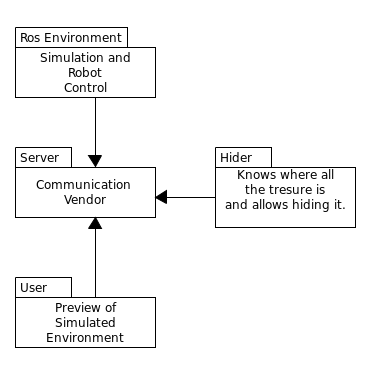
\includegraphics[width=0.7\textwidth]{figures/mainCommunication.png}
            \caption{Outline of the top level of communication.}
        \end{figure}

      With this main outline of communication done, it is also important to show how communication will be handled before it reaches a server. To do this the next two sections will talk about how communication is done in and out of ROS as well as how communication works in and out of the GUI.

      \subsubsection{Robot Operating system communication}
        ROS uses a published/subscriber mode of communication for its transfer of information. This means that while it is extremely simple to communicate between inside nodes, a new node will have to be developed that keeps communications to ROS to be switched on from outside sources. This can be viewed in the following figure:

          \begin{figure}[!ht]  
            \centering
              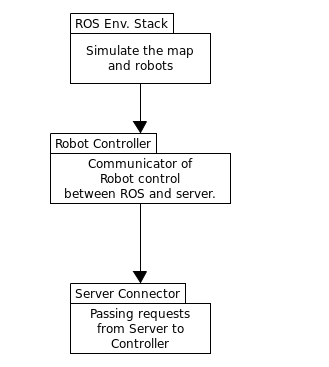
\includegraphics[width=0.8\textwidth]{figures/RosCommunication.png}
              \caption{Outline of the top level of communication.}
          \end{figure}

        The graph above presents a figure that shows that the communication starts at ROS Environment Stack. This has to be switched on for further channels that make sense. Then a robot controller node has to be created to ensure that sending goals is feasible when a command comes in but it shouldn't have direct connection to the server. The report has taken advantage of publisher/subscriber mode of communication and makes the server controller and robot controller contact in that exact manner. This actually allows for modularity between nodes as neither has to be switched on first and they can be changed and modified freely per users need. Considering that ROS codebase is done either in C++ or Python, with C++ proposing a better API in ROS environment, both nodes will be created using C++ and ran inside the same package that the simulation environment runs in to ensure maximum compatibility. This gives a good of idea of how the communication will be handled inside ROS. The next section will discuss how this communication is handled inside the Graphical User Interface environment.

      \subsubsection{Graphical User Interface/Hider Communication}
        In the Graphical User Interface, we can't take advantage of the Publisher/Subscriber approach that ROS loves to use. This means that while we can easily create both the user interface and the client that connects to the server. We need to think about how communication between the two will work to ensure that both writing and listening to the server is allowed and fires events based on responses. The same can be said for the Hider interface. This Hider interface could be implemented on the ROS environment stack alongside everything else but for the sake of modularity, the report will keep it outside. To develop this environment the following proposition is made for the environment:


        \begin{figure}[!ht]  
            \centering
              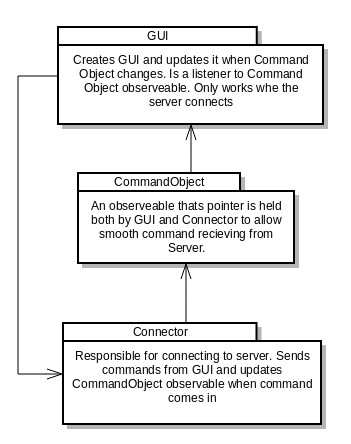
\includegraphics[width=0.8\textwidth]{figures/GUICommunication.png}
              \caption{Outline of communication inside GUI.}
          \end{figure}

        The Graphical user interface will implement an Observer design pattern to synchronize the communication between the GUI and the connector when a message comes in. The connector receives a command, changes the CommandObject and because the CommandObject was changes, the GUI as a listener will be fired and update the map. On the other side when the GUI wants to send a command, since it implements the Connector as a connection class, it should simply be able to pass the parameters directly into a command inside the Connector leaving the CommandObject strictly to the GUI to be fired when changed. With this, the report now has the design for the main protocol of communication and the next sections discuss the choices for design inside the ROS environment and GUI for the user.

    \section{ROS Environment}
      The most important consideration in design is scalability with which the simulations can run. In ROS we have two options for running the simulations one of which is Gazebo and the other Rviz for simulation preview. This is important to understand how the environment works and also if it actually works properly in terms of multi-robot environment.

      Each environment provides a certain ease of use inside the project with Gazebo allowing to build packages for robots making it a nice candidate for quick setup but also requires to constantly run Gazebo in the background which doesn't make it an ideal candidate for saving resources and performance which in the future might affect scalability. To avoid this issue, a better option would be to run Navigation Stack which is what will simulate the topics and the robot environment and to run Rviz for debugging purposes.

        \begin{figure}[!ht]  
          \centering
            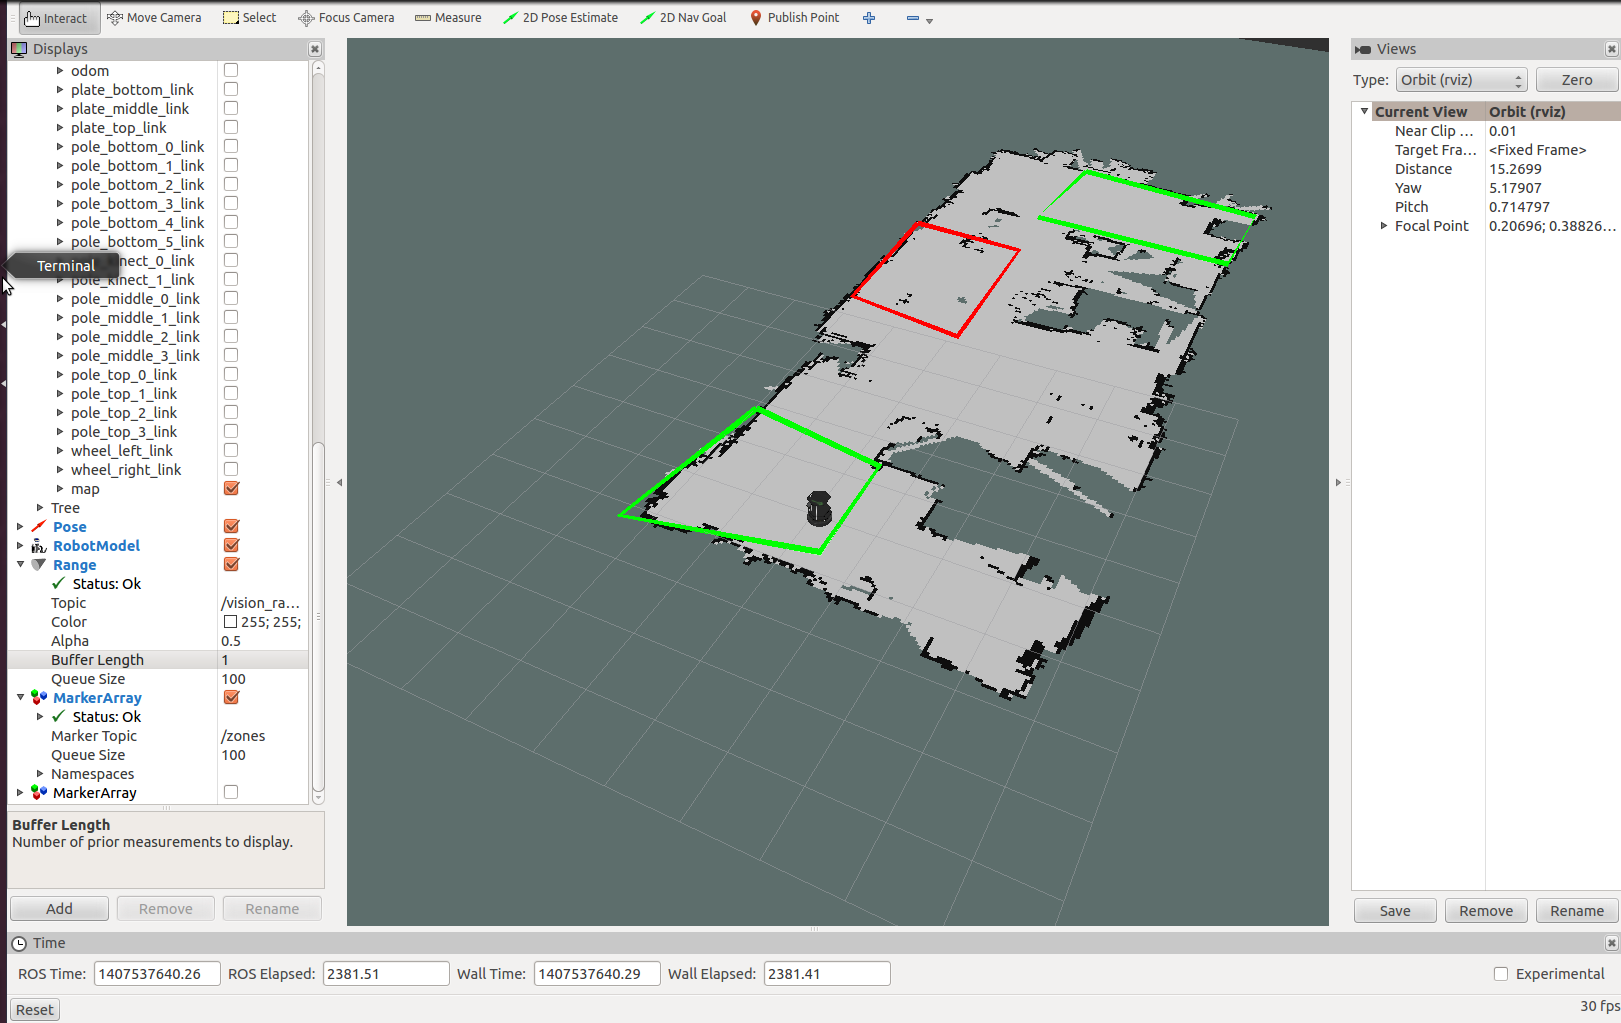
\includegraphics[width=0.6\textwidth]{figures/RVIZ.png}
            \caption{Example of Rviz running.}
        \end{figure}

      From current research, Rviz does not provide functionality in terms of displaying multiple robots but running it is optional in terms of environment so in that choice, Rviz is chosen to be the main simulation display in the first stages of the project. It will be used that when goals are set by the controller, the robot walks towards a certain path as well as ensure that the multiple layer design that ROS needs to implement in the navigation stack is chosen.

      To actually create multiple robot environment is a question of implementation and trial and error in the environment rather than design as the ROS navigation stack at this point is generally very unfamiliar however using answers provided in \cite{wiki1} we can imply that the design of the robot architecture will be as follows:

        \begin{figure}[!ht]  
          \centering
            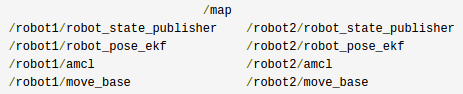
\includegraphics[width=1\textwidth]{figures/ROSPlan.png}
            \caption{Ideally how multi robot is going to work.}
        \end{figure}

      Figure above shows how two robots are mapped to the same map. The main challenge with this will be figuring out how to implement this in the Navigation stack without using gazebo for the backbone to avoid the need to consume extra resources through gazebo.

      It is important to note that originally the implementation will try to set up an environment with one robot that runs and allows to set up the GUI first. If however this doesn't pose too many issues, a two robot environment will be developed before the GUI is taken into consideration.

    \section{GUI for User and Hider}
      The GUI is the front of what the user sees and experiences through the use of application. This will be the main product that researchers will show to the users to later enquire about the dialogue model. It is therefore essential to ensure that the design is as simplistic and as intuitive as possible. After all the user should not feel like the design of the interface is in any way overwhelming. This could lead to not paying attention to the dialogue systems as well as bring on an experience that would otherwise compromise the flow of actions that lead the user from beginning to the end.

      While the previous section included an explanation of how the environment communicates with the server it did very little in explaining how the GUI is going to look or what programming language is going to be implemented to ensure both a pleasant experience for the user but also maximize compatibility with the Java Server that runs in the background and allows communication to the ROS environment. Both of these are discussed in the following sections.

      \subsubsection{The looks of the design}
        The application boasts quite a lot of information that the user needs to take in. The short list below summarizes most of the information that the user will see:
        \begin{itemize}
          \item The map and robots location on the map.
          \item List of possible robots that the user can select from
          \item Objectives of the game
          \item List of rooms that the robot can go to.
          \item Information about energy levels of various robots; each different.
          \item Dialogue windows popping up to start communication between robot and human.
        \end{itemize}

        With this list, a design can definitely start forming into shape with the last point being one of the most important ones. That the dialogues pop up rather than be placed in a sidebar or a top bar or anywhere else. The user should have a strong level of interaction with the robot as well as be able to make note of the communication that occurs. Once a robot gets a command it should communicate with the Human and notify them of possibilities or try to persuade them to do other things like go to another room or pickup a treasure that is distinct enough to others that it will be better to grab it rather than take a picture of the item if the user decides to take a picture of a distinct object.

          \begin{figure}[!ht]  
            \centering
              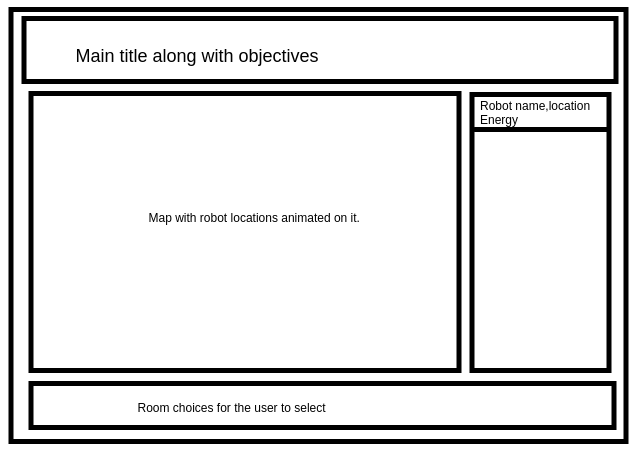
\includegraphics[width=1\textwidth]{figures/GUIDesign.png}
              \caption{Basic idea of the GUI design for the user.}
          \end{figure}

        This design largely represents the work flow of the application with the Dialogue window popping up requesting user input right in the middle of the frame to ensure that the user gives input to the robot and maximize the efficiency of the application.

        With regards to the hider GUI, it could be implemented as a GUI but creating a simple code that holds variables would make more sense as it will actually be faster to edit those than to do so through the use of GUI. It will keep external files to the minimum not requiring to run separate external files along with that .jar compiled file and with that rationale. At this point in the project it will suffice to have the Hider work at source code and change the variables inside it, compile and run accordingly.

      \subsubsection{Programming language choice}
        To develop the GUI itself, there are numerous options to choose from. Different languages offer different options and a list of possible programming languages taken under consideration in this report is:
        
          \begin{itemize}
            \item C++
            \item JavaScript
            \item Python
            \item Java
          \end{itemize}

        Each of these languages would be a good choice but to outline the main differences, each following chapter will discuss their positives and negatives.

        C++ is a great programming language for memory management and as such maximizing efficiency of the software through the use of pointers and memory dumping whenever any information is not necessary. With that, a graphical user interface could be set up in such a way that the user could execute a program and run it very easily. It does however bring a need to compile to specific operating systems like Linux, Windows or Mac depending on the platform that the software runs on\cite{cplus}. Also C++ has commands that are specific to each operating system meaning that while creating a C++ could potentially bring out the best performance, it would also create platform dependent binaries or even so, make code that is platform dependent and with that, it could potentially minimize the target audience for the project. Keeping the project as open platform as possible so that any user could run the GUI is also a very important aspect of the project.

        With JavaScript, the GUI would experience a very good boost in terms of GUI looks. Combining JavaScript with HTML could produce a very neat looking design that could update itself based on server output however the big issue with JavaScript is that it doesn't really support connecting to the server unless external platforms like socket.io\cite{socketio} are brought in. Otherwise JavaScript is AJAX dependent which means that it would either require an additional library importing and learning a new platform or, expanding the server to allow API calls but these kinds of implementations fall outside of the scope of possibility for this project.

        Python offers great ease of use, is a relatively fast language in comparison to the previously mentioned languages. It also works great with sprites and drawing GUI’s which could prove extremely useful in this project. This can be witnessed in books that teach Python programming and use sprite and GUI design as their main chapters\cite{python}. With python however, there is still an issue that was present with C++. While Python is an interpreted language, it works only if the interpreter is installed on the computer. With Linux based systems that is not an issue at all because Linux runs a lot of its software using Python so the interpreter is always pre-installed but when it comes to Windows, this interpreter is not installed as Windows tends to keep to its .exe file system and that again, would limit the scope for the audience.

        Java is the language that the Server was developed in. It is a language that has pre-built GUI libraries called Swing and AWT which allows for a fast GUI prototype implementation and is even use for general development in bigger corporations. These two are definitely favorable when it comes to the GUI created in this project. Java is also present on most PC’s because while systems don't use it as a pre-requisite, a lot of software is implemented using Java and there is a very high chance that any computer visited will have Java working on it. This provides a rationale for choosing Java for the implementation of the GUI.

    \section{Testing design}
      This project will taken upon itself a test driven development sprint where a set of criteria outlined in the specification will guide the way towards a successful implementation of the product. It is however important to outline some criteria other than the simplistic ones that are given in the specification for clarity purposes.

      One of these is to outline a use case for when the users are using the GUI to give an outline of what a successful implementation should do. With this user case, testing will later be carried out to ensure that the application has successfully undergone implementation purposes. Figure 4.7 demonstrates the basic use case that outlines the what the user should be able to do inside the application.

        \begin{figure}[!ht]  
          \centering
            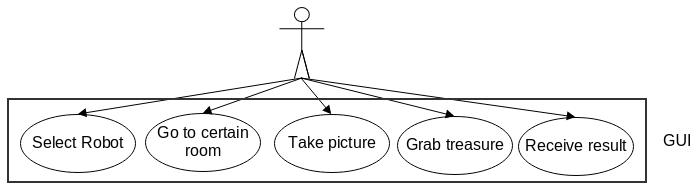
\includegraphics[width=1\textwidth]{figures/GuiUseCase2.png}
            \caption{Use Case for GUI.}
        \end{figure}

      With this we can see all the commands that are available to the user all of which should run successfully and without any issues.For a better explanation of the stages through which the application should go, a flow chart needs to be constructed. Such a flowchart will provide a better explanation of how the system works and in which areas lies logic that needs to be tested. Diagram presented in Figure 4.8 demonstrates the extent to which each logic function will need to be tested.

        \begin{figure}[!ht]  
          \centering
            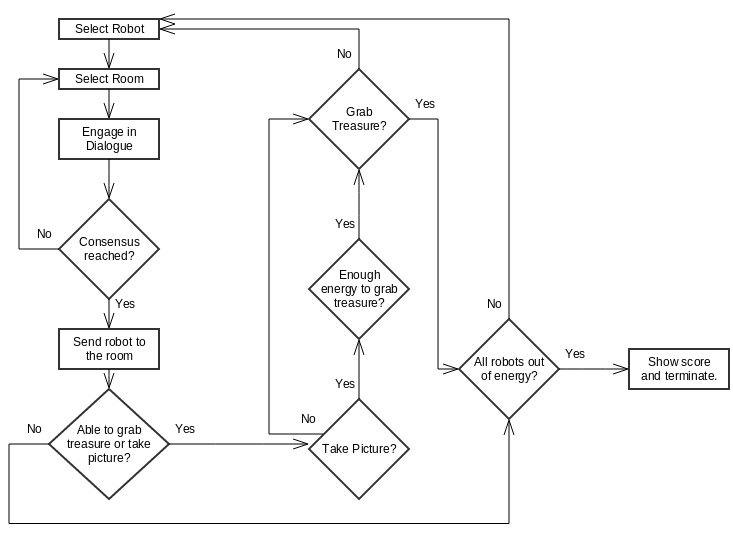
\includegraphics[width=1.1\textwidth]{figures/flowChart.png}
            \caption{Flow chart for GUI use.}
        \end{figure}

      It can be then implied that for the test driven implemented in this project, the application will need to reach the terminate state while ensuring that each decision in the use case has been tested. This will provide enough information to say that the product was fully finished along with the information provided in the specification.
\chapter{Implementation}
    The fully implemented product has been derived by the guidelines received from Elizabeth Sklar, King's College London who guided the implementation of the report and provided a Server package that in turn is now the main communicator of information of the finished product. This product can be broken down into several components these being(For a better explanation please refer to figure 1):
    \begin{itemize}
      \item Simulation Environment - A composition of packages composed of: Server Control, Robot Control and Robot Simulation.
      \item Server - A package composed of communication protocol classes.
      \item Hider - Composed of classes responsible for server connection and Hiding the treasures.
      \item User - Composed of classes responsible for UI, server connection and Remote Robot Control.
    \end{itemize}

    In following sections of this report, a more broken down structure to provide insight into how each of these is achieved.

    \section{Simulation Environment}
      As stated before, the ROS stack is a combination of three packages. The Server control, Robot control and robot simulation. They interact with each other in exactly the way that was stated in the design with Server control connecting to the robot control that then sends commands to the robot simulation however a more precise definition will be given in the next sections.

      The implementation also makes use of launch files to reduce the number of terminals that have to run during the execution of the simulation environment. This is due to the fact that with just the launch files given in the ROS tutorials, the amount of windows that have to be open for executing the environment can increase quite exponentially with the number of robots and is in no way automatic.

      This launch file further lists the important packages that implement the simulation and exposes user to the outline of how the ROS environment operates with further explanation of packages outlined in next sections of the implementation chapter.

      \subsection{The Server Control}
        The Server control implementation is based around creating a serverToController package outside of the ROS simulation. This is done to ensure that a modular approach was taken and the server can be extracted and replaced if such a need occurs. It also takes advantage of publisher/subscriber method to implement a workaround Observer Design Pattern that allows two classes to work together using callback functions rather than the Observer fire() events and implementing extra interfaces. This in turn, creates a much simpler to work with environment where the communication between two classes is transparent and callback methods are limited in their simplicity. It also implements C++ threads to allow socket connectivity through clients thus allowing a C++ server to connect using TCP client to the Java Sever running on currently a local host machine.

        The server control also ensures that no commands that are irrelevant to the Robot controller are sent through. This includes commands like \%\%ack or \%\%ping that only need to be answered by the server control. This in turn creates a sieve for commands from the server with only useful ones going through.

      \subsection{The Robot Controller}
        The robot controller is inside the same package that the Server control is based in. This is mostly to ensure that while modularity is kept, the classes aren't spread out so far inside an environment that it would make it difficult to troubleshoot. Also since these two nodes have a ROS topic that is dedicated only to themselves, it makes sense that they would be stored inside the same environment.

        The controller is used inside the ROS environment to communicate between the server commands and the robots themselves that are simulated and switched on along the server control and the controller. This controller send information to robot\/move\_base\/goal to send the robot a goal command that they need to reached. It has pre-programmed room numbers in a form of two separate array for x and y coordinates with the array positions representing room numbers for simplicity. This means that to access room 0, the program will look values up from x[0] and y[0]. A separate class could have been created to hold various rooms however creating and referencing objects in ROS can be quite tricky. It requires editing the CMake files and linking libraries for ROS automatic compiler that sometimes can get a bit buggy with ROS only allowing a handful of commands from the original C++ compiler.

        This can be very well seen when in the server control package as well as in the robot controller where the thread development was done through pThread class that C++ implements. There were other options online that allowed the same type of thread creation however a limited number of allowed C++ classes in the ROS stack has made it very difficult throughout the project to search for the ones that are allowed.

        Robot controller uses threads to ensure that when the goal is sent, the variables inside the thread are kept and unchanged(like which room was selected or which robot is it as identifiers would have to be broken down causing higher resource usage) during the robot reaching its goal. Since the method has to wait until a single robot comes back with a command that says that the goal has been reached, a thread was the perfect choice for this approach. This approach allows scalability and publishing to tf prefix topics was chosen to ensure that as many robots as possible can be controlled through this package.

        Once the robot has reached its goal that the thread was waiting for, a command is issued that published to a topic shared by the controller and serverToController that the package picks up using subscribe, calls back a method and later on sends it to the server. With this approach, the environment is never blocked concurrency wise but also makes the controller responsible for only the task that is controlling the robots.

        Finally, it is important to mention that currently the GUI does not allow altering the goals. This can be done, however it is important to note that when two subsequent threads are created for the same robot, the previous thread will get canceled and a message regarding reaching goal failure will occur. This actually makes sense because the changed goal means that previous goal is not reached however if a GUI is created that takes into account failure of reaching goals and allows altering them midway, it could pose issues for the developer that decides to create their own UI. Whenever a goal is altered then, a developer will need to be aware that they will receive a goal failed message and the previous node will die out to preserve resources.

      \subsection{The Simulation Environment}
        The simulation environment runs on an indigo version of ROS setup in Ubuntu. Most of the code has been developed using the Ros Wiki tutorials and as such some packages are directed in such a way to follow the standard set out by the ROS system. The system fully allows for multiple robots to exist on one simulation of the environment and takes advantage of the launch files to do so.

        All of the code for the ROS simulation environment is actually held in 2 separate packages. One package is for the environment and another is an exportable package holding classes for filling out the GridLayer.

        GridLayer was a plugin developed to create extra layers inside the costmap that is responsible for avoidance of obstacles inside the ROS environment. It's main motivation was to allow for robots to be notified of each others presence on the map and build planners accordingly to situations that might require each robot to avoid another. At this point in time, the ROS environment has a significant input lag that doesn't update the map in time for the robot to take advantage of the newly filled out layer. Updating the map in real time is actually quite unresponsive with occasional updates leading to a conclusion that at the time frame allowed for this project, updating the Grid Layer would not be feasible as it would require to go into the ROS environment and modify the codebase. This in turn would require a tremendous amount of resources.

        This however is not an issue for an environment that operates in real world rather than simulation as in real world the robot would build up its costmaps based on sensor input data that it receives. So while the project is in its works with regards to simulation, in future works that bug will turn out to be non existent and won't cause concern for the researchers. With that information, the implementation moved further.

        The other main package for the simulation contains nodes responsible for robot movement. Information like odometry, mapping of the topics as well as pose publishers are all present there and they are all edited so that they allow for multiple robots to run simultaneously and all be launched from a single launch file. This was achieved by doing two things: passing parameters to the robots with a certain robot number as well as including a tf\_prefix for specific robot groups so that the packages would not have to be reinvented. Such approach provides functionality that allows unlimited amount of robots to be launched using a launch file with only one visualization tool required to represent them.

        There is however a small issue to be addressed here. While the nodes are designed to work with as many robots as possible, the launch files that allow for fake localization are not quite as diverse and don't allow for parsing parameters to them. This is a challenge that the project encountered when trying to simulate the robot using the same fake localization files. It was later realized that fake localization uses topic names and as such configurations that are switched on but don't have their fields altered to include robot number prefix fail and create error reports at the start of the simulation.

        To go about this issue, extra launch files had to be created as that was the only way other than distorting the codebase to include configurations at the grouping. While this solution could be simpler it proposes a solution that is a whole lot messier and more difficult to keep up with if extra robots were added to the simulation. A suggestion of creating a package that generates the launch files can be drawn. It would require one parameter that takes in the amount of robots and with that generates all the logic so that the main launch file is also generated and running it, consecutively runs the simulation with the amount of robots specified. It is an easy solution however it falls outside of the scope of the project with regards to the time frame given. It is however a consideration to be taken on if the project was to be improved on.

        \subsubsection{Mapping in ROS}
        Mapping is the building block around the Robot Operating system. It works by mapping topics to other topics to make sense of the data. In the figure below we can see how the current implementation maps topics for a single Robot.

            \begin{figure}[htp]
              \makebox{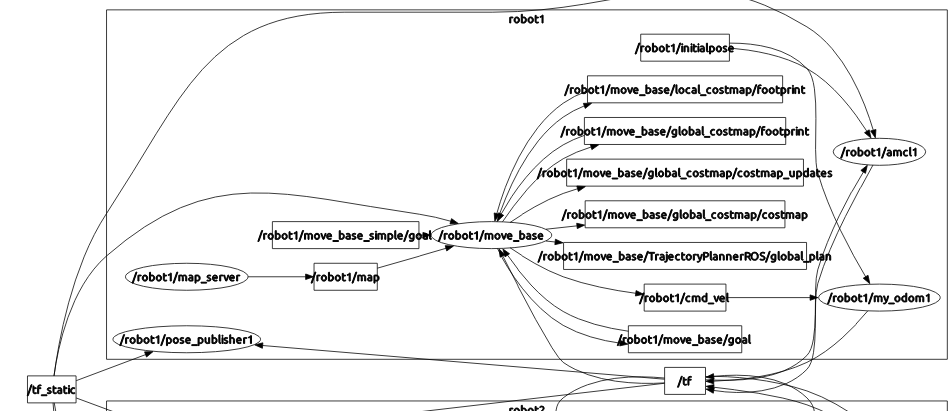
\includegraphics[width=1\hsize]{figures/ROSmapping.png}}
              \caption{Mapping of packages for a single robot.}
            \end{figure}

        This figure is only limited to topics that at the time of producing the graph were active. Several topics start to only publish at certain point like when a goal was reached so it goes to show how useful the launch files are and how many windows would otherwise had to be created to run all the topics separately.

        As previously stated ROS uses mapping to map certain topics to each other to be able to make sense of the data. Topics are generally nodes that publish any sort of data or can even be physical objects that map from one to another. This can for instance be mapping a robot hand to the body. This means that including a mapping graph gives a great deal of the implementation in the environment. The mapping graph however does not show which topics listen or publish data from and to each other and that's why in the previous figure, there is no connection between the goal node and the outside(not visible on this figure) controller node that would actually send data through about where the robot should go. Such graphs would be extremely complex and at larger levels unreadable.

        This figure then, was also included in the project to demonstrate the architecture behind how singular robots work inside the ROS environment. It lists every class developed in the Robot package along with those pre-build by ROS to aid in simulation. Perhaps the most important package inside the environment is the Odometry package that will be discussed further in the next section.

      \subsubsection{Odometry}
        Odometry is the use of data from sensors in robots to estimate their position in the environment. The location can never be exact as some things like slide or drag or friction when the robot is moving could slow it down causing a the estimation to go off if it doesn't take those into account and even then, the location will not be as accurate. In the simulation environment, this odometry can be considered to be very accurate and in the simulation package, odometry does very little in terms of robot estimation. This package in ROS, when ran is actually mostly used to collect velocity controls from the amcl that does the localization.

        AMCL is a probabilistic localization system for robots moving in 2D that implements a monte carlo localization approach through the use of particle filters. The science behind it is very complex and the implementation is done in ROS and available as a given package. As such it is unnecessary to further mention it than to explain that it is used for main planning using the map given and publishes velocities that the robots should take to ensure that it is in the correct position and that the amcl can follow its path.

        With this information, it is easy to infer that the odometry package for this project in ROS is responsible for accepting velocities and upgrading the robots pose by this estimation. Through that, it does follow the principle of holding the position but rather than the estimation mentioned in the definition, in the environment that is used as simulation this figure is much more precise.

        Odometry is also responsible for mapping of several topics and as such, it is one of the packages that is both a subscriber and a publisher. It subscribes to messages regarding velocities and publishes mapping required for the robot to move along the map and be visible to both the visualization software as well as amcl and move\_base that are responsible for implementing robot goals functionality. Some of these move\_base packages and amcl topics can be seen on figure 5.1.

        To make the odometry applicable to all the robots separately, there was a function implemented called getName that produces topic names based on the number received from the arguments. This simplistic approach allows for the same odometry node to be reproduced saving a lot of time with coding and compiling multiple odometries for each robot separately.

        For any future developers, it is important to note that Odometry that is present in the ROS Wiki pages at the time of writing the report does not implement any of the listening and publishing. It also moves the robot forward without any command given. There is even a lack of mapping the odometry to the robot which is not mentioned in the Wiki which for beginning developers might raise a lot concerns that their code is not working. This stalled the development of the environment by considerable amounts and with such a small community everything had to be worked out through trial and error.

        The next sections discuss in more detail how amcl and move\_base packages work for further understanding.

      \subsubsection{AMCL and move\_base packages}
        The amcl and move\_base packages are the packages that allow the robots to move through the plane in the current simulation environment. Without these, the robots would stand in place with no data. They connect the robot and odometry to the map and create obstacles based on the input data from the map. This in turn allows for maps to be created .png files and speeds up the process of rolling out new maps for the robots.

        They do however pose a certain difficulty when rolling out the robots. As previously stated these packages were not created to support multiple robots and they are implemented using yaml files that are static uncompiled interpreted files. This means that variable parsing is not allowed as it was with the odometry packages and separate files have to be created for separate robots. The solution to this was already discussed in previous sections.

        The move\_base package takes in five files in the current implementation all of which define the costmaps for each specific robot. This move\_base then creates the obstacles and allows the planning to be created for the robot and publishes cmd\_vel topics that were previously stated to be subscribed to by the odometry.

        This in turn creates defines the backbone for the robot environment with single robot environment explained in great detail. The next section outlines the how these packages together are taken to create a multi-robot platform.

      \subsubsection{Tf\_prefix and Multi-robot Functionality}
        It is important to note that tf\_prefix is considered deprecated in future releases of ROS due to developers not making good or any use of it with several packages starting off with the lack of support for tf\_prefix. However, it is also important to note that without it the project could not implement the multi-platform the way it did with a clean approach that allows to add robots using a simple checklist.

        The launch files in ROS take on a role of XML defined information sources for ROS to pull in and switch on nodes based on the information on them. This way rather than switching on topics like roscore and rviz, everything can be defined to be switched on automatically saving a lot of terminal windows being open. In this project, one launch file creates a two robot environment with server connections all in one terminal using only one command.

        This kind of approach using tf\_prefix allows for a list to exist that if followed to the letter will allow a developer to add a robot to the environment in an automatic way:
          \begin{itemize}
            \item Copy an existing groups XML code
            \item Increment all the arguments parsed by one
            \item Create separate local, global and common costmaps for this robot using the old ones and increment mappings by one.
            \item Direct move\_base parameters to these files
          \end{itemize}

        This short list allows for another robot to be created with ease. In the GUI all that has to happen is to increase the number of robots allowed to be selected in the source code and compile the code. This is to emphasize that the environment was created with customizability in mind. This section also summarizes in great detail the most important aspects of the implementation of the simulation environment. Further sections will discuss the challenges met along the way with implementing the simulation environment.

      \subsection{Challenges in simulation implementation}
        The implementation of this environment in 2D Ros was by far the longest process throughout this project. Due to ROS's continuous and rather violent growth a lot of Wiki's are outdated and the community tends to be very non responsive. A lot of the work that went into this had to be trial and error based with various packages working and not working through the development phases.

        Another note to make is that ROS implements its own version of a C++ compiler that does not contain all the packages that a regular user might wish to use especially when it comes to multi-threading. This became especially difficult to use when making plugins as referencing classes to each other turned out to be a very tedious and buggy process. Some plugins also turned out to spin(Ros uses spin to loop over topics and make callbacks based on each iteration) which made it impossible to subscribe directly to topics if that specific plugin was used. This made some of the development quite difficult especially the Grid Layer. Later on with testing it turned out that the Grid Layer couldn't process the information properly anyway which leads back to the point made about ROS's expanding growth and packages not being able to keep up. At the current moment ROS is an amazing architecture however at times one of its biggest challenges is that it makes it difficult for the developer to create clean readable code due to workarounds needed to push it to its full potential.

      \subsection{Final notes for Simulation Environment}
        A full implementation of the simulation environment runs using Rviz as a platform for testing whether the robots work. The navigation stack is fully implemented and accepts commands being taken in. The logging feature is switched on and ROS generally fills up on information quite fast so its absolutely essential that if used in the future, the developer should switch logging off unless they actually wish to troubleshoot. Otherwise ROS could overflow the drive quite fast after about 20-30 runs. Without logging these resources are well preserved and don't use up this much of the computers resources as no visualization software needs to be ran.

    \section{Server}
      While the server was fully implemented by  Sklar and Parsons\cite{technical}, it is the main tool that connects the environment and the GUI and with that, the commands and integration of this package into the system is important to discuss.

      The server can work on any operating system and will open up the Socket to computers connected in Local Area Network. If the computer enables connecting to it through the Internet using a dedicated IP, it would also be possible to host this server on a dedicated hosting machine that would then allow the environments to connect through the Internet and as such allow a much more flexible way using connections.

      This server accepts a big variety of commands to which explanations can be found in \cite{technical}. In this report however, only the commands that are used by the system will be discussed. These commands are:

        \begin{itemize}
          \item \textbf{\%\%setid} - When an application connects to the server it sets its id to receive messages from other applications.
          \item \textbf{\%\%ping} - Command sent by the server to applications to ensure that they are still connected.
          \item \textbf{\%\%pong} - Response to the ping command to confirm connection.
          \item \textbf{\%\%send} - Generic message send from application to application.
          \item \textbf{\%\%goto} - Command sent from UI to the simulation environment to move a robot to a place on the map.
          \item \textbf{\%\%found} - Command sent from UI to the Game master(In this implementation from hider to the UI) about information about location and characteristics of the server.
        \end{itemize}

      This outlines the commands used by both the UI and the simulation environment used in the current implementation. In the future sections, a discussion is created based on the conventions set by the technical description in \cite{technical} as well as an explanation of how each specific command is used in the implementation of the system.

      \subsection{Conventions}
        The server outlines some specific conventions by which the applications should connect to the server. These are by no way enforced however for ease of debugging they have been implemented in this system. This was also done to standardize how the system behaves. The name convention of apps connecting to the server are as follows:

          \begin{itemize}
            \item \textbf{SimR}: The simulation environment.
            \item \textbf{TabUI}: The GUI on the user side.
            \item \textbf{Hider}: The treasure knowledge base that holds information on which treasures are present in specific places.
            \item \textbf{Server}: The server running in Java.
          \end{itemize}

        It is also important to note that these names allow for generation of messages at source code level without having to create external files for what's the name of specific components in the system. Changing those at the current level of implementation would cause the system to malfunction and not deliver messages unless recompiled with changed names. For flexibility in the future, it could be possible to pass these as parameters in the main execution at terminal level or include external files.

        It is also important to note that the port used by the socket has been selected to be 6009. This is to inform that the server needs to be switched on with this specific port otherwise the applications won't be able to switch on properly. This port has been selected due to its availability and on most operating systems it is not used by any software so it is a safe option. On top of that it has been confirmed to guarantee complete data transfer on TCP level. It is only used be x11 windows server which generally does not use it anyway. With regards to threat it is not a targeted port so it keeps system security optimal. For information on this port please refer to \cite{port6009}.

      \subsubsection{Use of specific commands}
        This section outlines specific flows of data throughout the application to give a better image of how the server is being used. Each of those commands plays a specific role and there a demonstration of flow for specific situations is explained.

        \subsubsection{Connecting to the server}
          The connection to the server is fairly simple for Java while a bit more tricky for the C++. When Java connects it immediately sends a request to the server to set the id of the application(Using the \%\%setid command). It then receives an ack command that can be ignored and simply confirms that the id has been set by the server. If the socket doesn't exist, the application terminates. If the application receives a shutdown command it will still work for demonstrative purposes of the application but this only happens if the application was switched off and didn't give server time to clean out the old id that will not respond to the next ping request.

          This works in a similar manner to C++ however with C++, there is almost no way to deal with the server not connecting and the C++ will start to complain about lack of existence of to the server filling up a big chunk of the ROS logging utility and take up drive space. The only way is to set a timeout to connecting to the server however that will also slow down the flow of information so before switching the simulation environment, it is best to start up the server or to comment out the node packages responsible for connecting to the server in case of testing the environment.

        \subsubsection{Sending a robot to specific location}
          Normally it is possible to send the robot to any location using x and y coordinates but in the current implementation of the system these are hard coded at the simulation environment. This means that rather than using the standard goto command that accepts x and y coordinates, the x and y coordinates are both set to the room number the robot is finished. It would be better to use only one argument for the room number but at this point in time the server is very specific about the number of arguments it receives. This then is passed through the server to the simulation environment and the robot is sent traveling to a specific room.

        \subsubsection{Robot reaching the goal}
          When a robot reaches its goal, the environment sends a generic message in the form of "robotNo;roomNo". This message is very easy to understand and when a client receives a message of type send with these arguments it updates the map and starts initializing the dialogue for taking the treasure.

        \subsubsection{Asking about the treasure}
          To receive the first information about the treasure the client sends a quick message to the Hider class and waits for a response before showing user the dialogue. This request is sent as soon as the UI receives the news of robot reaching its goal for efficiency. This message is a generic send message sent to the hider with a room number as an argument. In the hider this message is easily decrypted and a reply is sent using a found type message that contains the details about the treasure.

      \subsection{Final notes about the server}
        The server is a great piece of work that saved a lot of time during the implementation of the entire system. With it the environment only has to connect, set an id and the messages are being send back and forth without a problem. There are small issues like the time it can take to clean up old clients to reconnect again but that would consume resources on a computer and would not really affect the working system as much. It is only useful for testing.

        Another big note to add is that the server at the time of implementation notify a client of a message being sent successfully or failing to do so because some other client disconnected. This means that troubleshooting is more difficult as this type of lack of responses leads to having to develop more generic messages that could make the system more complex and messages have to be generated at both sides rather than simply filtered.

    \section{Hider}
      The hider is a very simple two class package that implements a very similar approach to the UI which will be explained later. Currently it holds a HashMap of treasures with an Integer acting as a key to each specific room. When a command comes in, the Hider looks to the HashMap which have a lookup time of O(1) retrieves the treasure details and send those back to the UI.

      The implementation of the Observer design pattern here allows for the main Hider class to be a listener to the server and as such whenever a request comes in, the Hider implements it without a problem.

    \section{User}
      As stated in the design section, the User UI was developed using Java Swing interface to save as much time as possible before rolling out a fully released 
\chapter{Professional and Ethical Issues}
Either in a seperate section or throughout the report demonstrate that you are aware of the \textbf{Code of Conduct \& Code of Good Practice} issued by the British Computer Society and have applied their principles, where appropriate, as you carried out your project.

\section{Section Heading}

\chapter{Evaluation}
    \section{Project Progress Evaluation at the time of report}
      This section will largely focus on evaluating the progress made during the report. It will discuss the original goals against what was achieved and what was missing in the project. What things could have been done better? What things have been done well? Why have some things not worked out quite the way they should(Think robots overlapping each other or not constantly upgrading the map or robots not proposing what rooms to go to). Also discuss the help that was reached out for and critique the ROS community as they are difficult at times. Discuss where the project could be applied? Also make a note how compared to real life this map was really small and usually robots will have much bigger environments to transverse through. This means that if time is of essence, supporting multiple robots is absolutely critical and being scalable is another issue to look at which the project did focus on in code design.

    \section{How the project compares with other research}
      Following that, discuss how this project compares to other papers previously stated in the background and as such. In what way was this project something completely different(Think humans not in the same environment as robots). How was it similar?(Think about the collaboration papers focusing on fluency). For more ask at tomorrows meeting what can be discussed here. I could also discuss the inverse property of the project against projects like Amazon Drone Delivery.

    \section{Future possibilities for expanding the project}
      Should I write something here?

      \subsubsection{Minimizing dependencies}
        Complete care was given in the project to made the code as scalable as possible through the use of non discriminating functions(Functions that apply to all robots) through Object Oriented Programming etc. But some functions in ROS do require the user to create separate file for each robot and as such, more elaborate ways could be thought of to allow a more Object Oriented approach to be taken. With that, the scalability of the project could increase to the point that it would turn more into a non-deterministic framework that allows plug-ins to be taken in.

      \subsubsection{Automatic area clustering of robots}
        Based on research done in Sensor networks, energy limitations are a huge concern there and multitude of research was carried out on maximizing the lifetime of networks. As such, motivation can be given to displacing the robots throughout the map to maximize their lifetime and guide the user better around the game. This could be done through the use of clustering algorithms for robots to negotiate on which part of the map they will focus on. In this project this will take on a bigger challenge as in some scenarios where environments are hostile robots could be lost along their path and as such two robots could agree to search regions of the map.

      \subsubsection{Start using physical robots for the Game}
        The project stopped at using simulations to run the game. In this way it is not much different than using simple game software to simulate such an environment. Creating a framework using ROS actually allows the project to transfer from simulation to real life is actually fairly straightforward with the foundations already built up. With the robot controller, all functions are sent to specific robots odometry and since odometry will always be present the next focuses in the project could be to start implementing real life robots with maps uploaded onto them.

        In such scenarios a lot of issues would be overcome with robots creating real time data and submitting them to the map as well as avoiding obstacles that could be other robots. In such a case study users would have access to robots but not see the maze themselves. It would add excitement to the game.

      \subsubsection{Expand the GUI to JavaFX}
        Currently, the GUI is built using Java Swing which in itself is a very formal language that is usually used to build business like components with little support for drawing extra objects or on panes. There are packages such as AWT but their use is widely discouraged by the community and could stall the project more.

        Instead a proposition of using JavaFX is in place. This package is slowly used more frequently to add flexibility to otherwise difficult to handle Java GUI design. In the end the projects audience is what will determine the projects quality so ensuring a solid GUI could be the way to move forward.

      \subsubsection{Add Phone support}
        While a minor feature requiring to only boot up another GUI, gaming on the phone is becoming more and more of a standard. With that in mind giving users the freedom to not carry around a laptop to events where the game might be played, using hotspot routers for the game and allowing applications to play the game on top of computers could be in fact a very useful feature. There are numerous possibilities for implementing such a feature but there are also technologies that allow writing applications that export to all phone platforms. Discussing them however falls outside of the scope of the project.

      \subsubsection{Flexibility through Multi ROS Support}
        If the environment stayed as it is, creating VM's that run multiple ROS environments and handle them accordingly could be an approach to create a gaming environment that multiple users could enjoy online whenever they would choose to wish so. Such environment would work by using name assigning and would require adding another Server node that would handle multiple instances of the current server class that would populate itself over the machines ports with sockets. 

        This would create a scalable game environment that potentially an unlimited number of users could use. This could open opportunities for competitions in the game where based on a scoring system of choice users could compete in robotics challenges that use actual real robot operating system as opposed to simulations that wouldn't otherwise give them an experience of using a \"real\" robot in its environment.
      
      \subsubsection{Deep sea exploration}
        ROS currently lacks the support for 3D path planning. This is not to say that 3D control, that is actually available but in the future, plans might extend to ros being able to support 3D path planning and then another world of opportunity will open up in Deep sea exploration. The current project allows for communication between ROS and whatever GUI is presented so its not difficult to see how inputting the right packages for such implementations could be extremely useful. Already a lot of research has been going into node deployments in deep sea and how to use these to tackle communication however, map building of deep sea ocean and understanding more about what's beneath us is an area of research that could benefit from the framework suggested in this project where robots are given coordinates through a server allowing for a customizable GUI on the side of developers for such projects.

      \subsubsection{Search-And-Rescue Scouting}
        This is actually an extension to the paper by Govindarajan\cite{Vijay} where robots would assist a person to minimize time spent in a single room during search and rescue missions. This project could be an extension to that but much rather use robots for pre-made environments that suffered some kind of trauma to weight risks of assisting certain people and search for survivors in places that have the best chance of making it out. Building maps of risky environments could give rescuers chances of creating robust plans that would maximize the number of people saved in such harsh and difficult times.
\chapter{Conclusion}
In this project, a dialogue-based framework for human robot collaboration was created. With the use of ROS simulation package as well as a complete Java GUI design it is now possible to research how people would respond to environments that closely resemble those running in real life and as such produce a standardized work kit for argumentation-based dialogue research. Developing a solid framework that incorporates various programming platforms proved to be difficult due to time constraints but through careful and systematic approach proved to be possible.

The project was inspired by Sklar and Azhar's\cite{Elizabeth} paper on Argumentation-Based Dialogue Games for Shared Control in Human-Robot Systems and is a direct implementation of the game proposed in the project with a different UI approach. The project was also used as a measure of learning and expanding the field of knowledge with regards to Robotics development and integration development which it succeeded in greatly.

%%%%%%%%%%%%%%%%%%%%%%%%%%%%%%%%%
% References
%%%%%%%%%%%%%%%%%%%%%%%%%%%%%%%%%
\bibliographystyle{plain}
\bibliography{references}
\addcontentsline{toc}{section}{Bibliography}

%%%%%%%%%%%%%%%%%%%%%%%%%%%%%%%%%
% Appendices
%%%%%%%%%%%%%%%%%%%%%%%%%%%%%%%%%
\appendix
\include{Appendices/appendix}
\chapter{User Guide}
	\section{Guide for game users}
	This guide is aimed at users that might have to switch on the game and follow basic steps to play it. It does not incorporate any admin knowledge and switching on the other parts of the game. That will be outlined in the next chapter.(To see the application in action you can also watch the video on \cite{Dialogue full implementation})

	To start the game you will need to find the package and run it. This is done by simply switching on the GuiUser package from terminal using the jar command for Java. If you see the following message: 

	\begin{figure}[htp]
		\centering
		\makebox{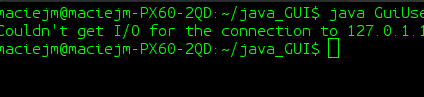
\includegraphics[width=0.4\hsize]{figures/IOError.png}}
		\caption{Input Output error from the server.}
	\end{figure}

	It means that the server is down and you need to contact the application administrator to get it up before you can run the game. If that has happened you will be presented with the following screen:

	\begin{figure}[htp]
		\centering
		\makebox{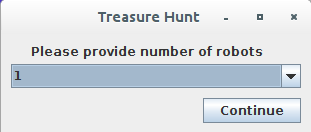
\includegraphics[width=0.4\hsize]{figures/App1.png}}
		\caption{Number of robots prompt.}
	\end{figure}

	This means that the application is ready to start playing the game. If you select the number of robots you should then be presented with the following screen:

	\begin{figure}[htp]
		\centering
		\makebox{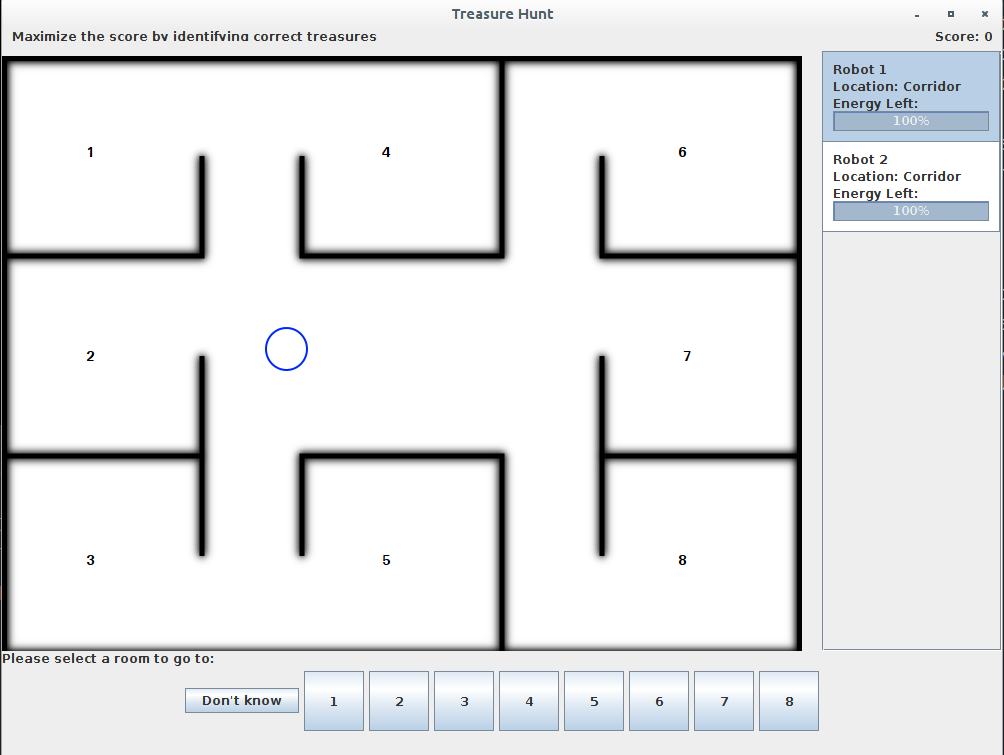
\includegraphics[width=0.4\hsize]{figures/finished.png}}
		\caption{Full GUI.}
	\end{figure}

	This is the UI interface from which you can play the game. Once you select a room a robot will engage in a conversation with you whether or not you wish to visit the room: \\
	\begin{figure}[htp]
		\centering
		\makebox{
\includegraphics[width=0.4\hsize]{figures/App2.png}}
		\caption{Dialogue prompt}
	\end{figure}
	If so, the robot will set itself to a traveling state until it reaches that room. \\
	\begin{figure}[htp]
		\centering
		\makebox{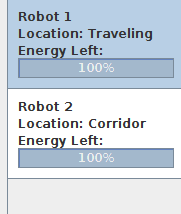
\includegraphics[width=0.3\hsize]{figures/App3.png}}
		\caption{Robot traveling.}
	\end{figure}
	You can also select another robot if you selected more than one robot to control at the start. If that's so please notice that the room that you sent your previous robot to will not be click-able. This just means you can choose each room once so choose wisely.
	\begin{figure}[htp]
		\centering
		\makebox{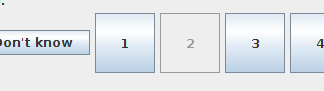
\includegraphics[width=0.3\hsize]{figures/App4.png}}
		\caption{Room no longer click-able.}
	\end{figure}
	Once the robot arrives to its destination. You will be prompted about the treasure footprint and colour that the robot discovered. You will be able to choose a treasure from a set of desired ones. These treasures will closely identify to the colour or footprint so you can make the decision now or take a picture.
	\begin{figure}[htp]
		\centering
		\makebox{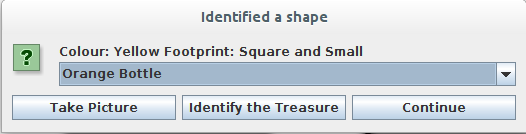
\includegraphics[width=0.3\hsize]{figures/App5.png}}
		\caption{Prompt regarding robot finding the treasure.}
	\end{figure}

	Before clicking identify the treasure you should always make sure that you select a treasure from the drop-down list first otherwise the first selection on that list will be carried out which would not be ideal. Remember that taking pictures costs so try to minimize the need to do so. For now take a picture for learning purposes.

	\begin{figure}[htp]
		\centering
		\makebox{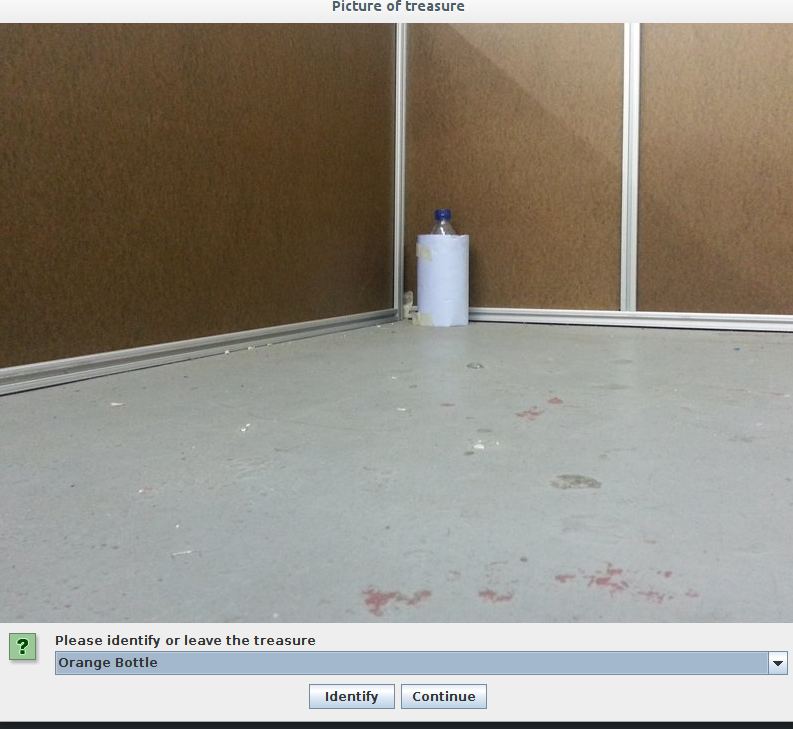
\includegraphics[width=0.3\hsize]{figures/App6.png}}
		\caption{Effect of taking a picture}
	\end{figure}

	You are now presented with a picture of the treasure and should be able to deduce what you are seeing but you can still press continue to forfeit the treasure. If you however identify and treasure you will receive a reply similar to this one:

	\begin{figure}[!htp]
		\centering
		\makebox{
\includegraphics[width=0.3\hsize]{figures/App7.png}}
		\caption{Successful identification}
	\end{figure}

	Continue the previous steps and try to maximize the score as well as visit all the rooms. When you either visit all the rooms or the energy runs out from your robots you will finish the game. At that point you will receive the following type of message:
	\begin{figure}[htp]
		\centering
		\makebox{
\includegraphics[width=0.8\hsize]{figures/App8.png}}
		\caption{Game finished.}
	\end{figure}

	This will conclude the user guide for playing the game.

	\section{Admin Guide}
	This guide is aimed towards a person that has already set up the environment and looks to customize the program a little bit or start modifying it to their needs. It includes information on handling templates and how these templates are used in the program. It also says where to look for debugging tools in the software to ensure that there is a full coverage of information starting with the basics.
		\subsection{Templates}
		The GUI software boasts three templates in its system each of which contains information by which the program runs. You can edit each of those by a specific set of commands.\\
		\textbf{mapTimes template}: This is by far the most difficult template to get right but if eventually done it allows for customized cost creation for the robots. It is in a form of the first line containing the number of nodes in the matrix with the following lines being costs of x and y in the form of 'from' to 'to'. For a better understanding you can use the following figure:
		\begin{figure}[!htp]
		\centering
		\begin{tabular} {l}

			9 \\
			99 17 14 17 13 13 16 13 15 \\
			99 99 18 23 10 19 21 18 21 \\
			99 17 99 18 15 14 19 17 19 \\
			99 23 22 99 18 10 22 19 21 \\
			99 18 22 26 99 26 22 22 29 \\
			99 26 21 17 21 99 22 20 24 \\
			99 29 27 29 24 24 99 16 21 \\
			99 24 24 26 20 20 15 99 17 \\
			99 27 27 29 24 25 23 18 99 \\
		\end{tabular}
		\caption{Map Adjacency matrix}
		\end{figure}

		\textbf{DialogueText template}: This template is responsible for the type of questions you may want to ask your users when you present them with a GUI and allows for the dialogue between the robot and the user when a room is selected to go to to make sure that's what the user wants. This template follows a convention. The first line in the template defines the name of the template, the next lines until "SpecificRoom:" line are responsible for asking the users questions that relate to not being sure. Following the Specific room line are questions that you want to ask the user with regards to selecting a specific room. There is also built-in support for two reserver words that will be replaced with actual values in the environment. These values are £room£ and £cost£ both of which mean their implied meaning which is the room that the user wants to visit and the cost to get there. An example of the following template can be:

		\begin{figure}[!htp]
		\centering
		\begin{tabular} {l}
			DontKnow: \\
			Do you want me to go to room £room£ \\
			It will cost me £cost£ to go to room £room£ \\
			Are you sure? \\
			SpecificRoom: \\
			It will cost me £cost£ to go to room £room£ \\
			Are you sure? \\
		\end{tabular}
		\caption{Dialogue template}
		\end{figure}

		This template is currently used by the developed environment.
		\textbf{treasures template}: This template exists in two versions and follows a simple standard. That is the first line represents the number of rooms on a map. The hider uses this value to determine the number of treasures to disperse. The lines following this one are treasure descriptions each of which follows the same format. That is: \{Colour, Footprint, Points, What the treasure actually is, Filename\}. These values of comma separated and don't hold any parenthesis. If parenthesis will be used they will be treated as part of the treasure description. The filename is omitted in the template used by the GUI so whenever editing one make sure to change it in the GUI as well for compatibility reasons.

		\section{Running the application}
		The application is extremely easy to start on the environment that already supports it. To run the full stack, navigate to respectable folders of the implementation in the terminal and type the following commands to run the full system:
		\begin{itemize}
			\item \$ java Server 6009
			\item \$ roslaunch robot launch\_robot.launch
			\item \$ java Hider
			\item \$ java GuiUser
		\end{itemize}
		If the execution went correctly then the Server should produce a list of clients connected. Together it should connect TabUI, Hider and SimR. If you wish to debug at any point you can always use the Rviz package inside ROS. At the time of delivery it was left switched on so if you'd like to switch it off please use comment it out in the launch\_robot.launch file inside the Ros package robot.
\chapter{Source Code Listings}

I verify that I am the sole author of the programs contained in this file except where explicitly stated to the Contrary.
Your Maciej Musialek 25/05/2016.
\lstset{frame=tb,
  language=Java,
  aboveskip=3mm,
  belowskip=3mm,
  showstringspaces=false,
  columns=flexible,
  basicstyle={\small\ttfamily},
  numbers=left,
  numberstyle=\tiny\color{gray},
  keywordstyle=\color{blue},
  commentstyle=\color{dkgreen},
  stringstyle=\color{mauve},
  breaklines=true,
  breakatwhitespace=true,
  tabsize=3
}
\section{Gui And Hider source code}
\subsection{Main GUI Class}
This class is responsible for the main communication inside the User folder. Its folder path therefore is: \\GuiUser.java
\begin{lstlisting}
//GuiUser.java
import java.util.*;
import java.io.*;
import javax.swing.*;
import java.awt.event.*;
import java.awt.*;
import javax.swing.table.*;
import java.awt.image.BufferedImage;
import javax.imageio.ImageIO;
import javax.swing.event.*;
import java.beans.*;
/** 
	A class responsible for holding user data and listening to specific events
*/
public class GuiUser implements Listener{
	//Just a starter method for GUI with basic CLI.
	CommandObject command;
	Connector r;
	Robot[] robots;
	JComboBox<String> noRobotsBox;
	int i;
	JButton[] rooms;
	int selectedRobot;
	int firstSelection;
	JTable table;
	GUI gui;
	JPanel mapPanel;
	JLabel map;
	DefaultTableModel tmodel;
	ArrayList<Integer> unvisitedRooms;
	Dialogue dialogue;
	int takePictureCost;
	int grabTreasureCost;
	boolean consensus;
	int curQuestion;
	int score;
	ArrayList<String[]> treasureOptions;
	String[] actualTreasOptions;
	JLabel scoreLabel;

	//Starter method
	public static void main(String[] args) {
		new GuiUser();
	}
	//Constructor for all the basic commands and server initialization.
	public GuiUser() {
		score = 0;
		firstSelection = 0;
		takePictureCost = 10;
		readInTreasuresAndRoomsAmount();
		command = new CommandObject();
		addListener(command);
		this.r = new Connector("127.0.1.1", 6009,command);
		Thread r2 = new Thread(r);
		r2.start();
		waitForServer(r);
		r.setId("TabUI");
		gui = new GUI();
		
	}
	//Implementing Listener Interface
	public void addListener(CommandObject command) {
		command.add(this);
	}

	//An empty blocking method that ensures that server has time to set up before continuing running asynchronously.
	public static void waitForServer(Connector r) {
		while(!(r.isRunning())){
			System.out.print("");
		} //Wait for the server to start up before continuing.
	}

	//Simple method that sends a send robot message and asks the server to pass it through.
	public void sendRobot(Connector r, int robot, int room) {
		int costOfTravel = dialogue.getCost(robots[robot].getRoomNumber(), room+1);
		robots[robot].setCost(costOfTravel);
		robots[robot].setTraveling(true);
		r.sendMessage("%%goto TabUI SimR " + robot + " " + room + " " + room + " 45");
		unvisitedRooms.remove(new Integer(room+1));
		dialogue.setUnvisitedRooms(unvisitedRooms);
	}

	//Just a command ran occasionally to ensure that the game ends.
	public void checkIfGameFinished() {
		int blockedRobots = 0;
		for(int i= 0; i<robots.length;i++) {
			if(robots[i].getBlocked()) blockedRobots++;
		}
		if(blockedRobots == robots.length) gui.showFinishSplashDialog(false);
		else if(unvisitedRooms.size() == 0) gui.showFinishSplashDialog(true);
	}

	public void readInTreasuresAndRoomsAmount() {
		ArrayList<String> tempTreasArray = new ArrayList<String>();
		treasureOptions = new ArrayList<String[]>();
		try (BufferedReader br = new BufferedReader(new FileReader("treasures"))) {
		    String line = br.readLine();
		    while ((line = br.readLine()) != null) {
		       String[] temp = line.split(",");
		       tempTreasArray.add(temp[3]);
		       treasureOptions.add(temp);
		    }
		} catch(FileNotFoundException e) {
			System.out.println("File not found.");
		} catch(IOException e) {
			System.out.println("IO Exception");
		}
		actualTreasOptions = new String[treasureOptions.size()];
		actualTreasOptions = tempTreasArray.toArray(actualTreasOptions);
	}
	//Send a message to ask about the treasure
	public void askForTreasure(int room ) {
		r.sendMessage("%%error TabUI Hider  \""+room+"\"");
	}
	//Regirter and unregister implementations of the Listener class
	public void register(Observable observable) {observable.add(this);}
  	public void unregister(Observable observable) {observable.remove(this);}

  	//Calculate all the new attributes of the robot.
  	public void fieldChanged(Object source, String attribute) {

    	if(attribute.contains("error")) {
    		updateRobot(attribute);
    	}// this has to be implemented
    	else if(attribute.contains("found")) {
    		gui.createDialogs(attribute);
    	} else if(attribute.contains("score")) {
    		String recievedPoints = attribute.split(",")[1];
    		recievedPoints = recievedPoints.substring(0,recievedPoints.length()-1);
    		gui.showMessage(Integer.parseInt(recievedPoints));
    		
    		score += Integer.parseInt(recievedPoints);
    		scoreLabel.setText("Score: " + score);
    		checkIfGameFinished();
    	} else if(attribute.contains("image")) {
    		String[] brokenDownCommand = attribute.split(" ");
    		String filename = brokenDownCommand[brokenDownCommand.length-1];
    		int room = Integer.parseInt(brokenDownCommand[brokenDownCommand.length-2]);
    		robots[selectedRobot].setCost(takePictureCost);
    		robots[selectedRobot].subtractCost();
    		gui.takePicture(filename,room);
    	}
  	}

  	//Update robot values after it reached its goal.
  	public void updateRobot(String attribute) {

  		//Split up the message
  		String[] temp = attribute.split("\"");
		temp = temp[1].split(";");

		//Send a message regarding the treasure
		askForTreasure(Integer.parseInt(temp[1]));

		//Update the robot information
		int robotId = Integer.parseInt(temp[0]);
		robots[robotId].setLocation(Integer.parseInt(temp[1])+1);
		robots[robotId].setTraveling(false);
		robots[robotId].subtractCost();

		//Change the maps and update the table
		if(selectedRobot == robotId) gui.updateMap(robots[robotId].getRoomNumber());
		tmodel.fireTableDataChanged();
		table.changeSelection(selectedRobot, 0, false, false);
  	}
  	//Class responsible for creating the GUI and handling its logic.
  	private class GUI extends JFrame{
  		
  		private static final long serialVersionUID = 1L;

		public GUI() {
			super("Treasure Hunt");

			unvisitedRooms = new ArrayList<Integer>();
			for(int i = 1; i<9; i++) {
				unvisitedRooms.add(i);
			}
			dialogue = new Dialogue(unvisitedRooms);
	        this.setDefaultCloseOperation(JFrame.EXIT_ON_CLOSE);
	 
	        JLabel emptyLabel = new JLabel("");
	        emptyLabel.setPreferredSize(new Dimension(175, 100));
	        this.getContentPane().add(emptyLabel, BorderLayout.CENTER);
	 
	        //Display the window.
	        scoreLabel = new JLabel("Score: " + score);
	        buildRobotAskingPanel();
	        this.pack();
	        this.setVisible(true);
		}

		//This message tells the user whether or not their identification was correct.
		public void showMessage(int score) {
			if(score>0) {
    			JOptionPane.showMessageDialog(this, "Identification Successful: " + score + " points", "Success", JOptionPane.INFORMATION_MESSAGE);
    		} else {
    			JOptionPane.showMessageDialog(this, "Identification Unsuccessful: " + score + " points", "Attempt Failed", JOptionPane.INFORMATION_MESSAGE);
    		}
		}
		//Beginner Screen to select the amount of Robots the user can use.
		public void buildRobotAskingPanel() {
			JPanel container = new JPanel();
			container.setLayout(new BoxLayout(container, BoxLayout.PAGE_AXIS));
			JButton continueBtn = new JButton("Continue");
			String[] noRobots = { "1","2"};

			noRobotsBox = new JComboBox<String>(noRobots);
			noRobotsBox.setSelectedIndex(0);

			continueBtn.addActionListener(new ActionListener(){

				public void actionPerformed(ActionEvent e)
	            {
	                //Execute when button is pressed
	            	String temp = String.valueOf(noRobotsBox.getSelectedItem());
	            	robots = new Robot[Integer.parseInt(temp)];
	                buildMainPanel();
	            }


			});
			
			//Lay out the label and scroll pane from top to bottom.
			JPanel listPane = new JPanel();
			listPane.setLayout(new BoxLayout(listPane, BoxLayout.PAGE_AXIS));
			JLabel label = new JLabel("Please provide number of robots");
			listPane.add(label);
			listPane.add(Box.createRigidArea(new Dimension(0,5)));
			listPane.add(noRobotsBox);
			listPane.setBorder(BorderFactory.createEmptyBorder(10,10,10,10));

			//Lay out the buttons from left to right.
			JPanel buttonPane = new JPanel();
			buttonPane.setLayout(new BoxLayout(buttonPane, BoxLayout.LINE_AXIS));
			buttonPane.setBorder(BorderFactory.createEmptyBorder(0, 10, 10, 10));
			buttonPane.add(Box.createHorizontalGlue());
			buttonPane.add(continueBtn);

			//Fill out the container.
			container.add(listPane, BorderLayout.CENTER);
			container.add(buttonPane, BorderLayout.PAGE_END);
			this.add(container);
		}

		public void buildMainPanel() {
			//Create a new container
			JPanel container = new JPanel();
			
			//Let's start the robots off.
			for(int i=0; i<robots.length; i++) {
				robots[i] = new Robot("Robot " + (i+1), i, 100, "-1");
			}

			//Introduce the main panels.
			JPanel topLabelPanel = new JPanel(new BorderLayout());
			mapPanel = new JPanel();
			JPanel robotList = new JPanel();
			JPanel roomOptionList = new JPanel();
			JPanel middlePanel = new JPanel();
			JPanel bottomPanel = new JPanel();

			//Set their sizes.
			topLabelPanel.setPreferredSize(new Dimension(1000,20));
			mapPanel.setPreferredSize(new Dimension(800,600));
			robotList.setPreferredSize(new Dimension(180,600));
			roomOptionList.setPreferredSize(new Dimension(800,100));

			tmodel = new DefaultTableModel();
			tmodel.addColumn("NoHeader", robots);
			//Fill out the robotList
			table = new JTable(tmodel) {
				 private static final long serialVersionUID = 2L;
				 public boolean isCellEditable(int row, int column) {return false;}
			};
    		table.setDefaultRenderer(Object.class, new RobotRenderer());
    		ListSelectionListener cellsChange = new ListSelectionListener() {
    			public void valueChanged(ListSelectionEvent e) {
    				if (e.getValueIsAdjusting()) return; 
    				int temp = ((DefaultListSelectionModel) e.getSource()).getMinSelectionIndex();
    				if(temp != -1) {
    					selectedRobot = temp;
    					firstSelection = temp;
    				}
    				else selectedRobot = firstSelection;
    				updateButtons(robots[selectedRobot]);
    				updateMap(robots[selectedRobot].getRoomNumber());
    			}
    		};

    		table.getSelectionModel().addListSelectionListener(cellsChange);
    		table.setTableHeader(null);
    		table.setRowHeight(90);
    		robotList.setLayout(new BorderLayout());  
    		robotList.add(new JScrollPane(table));   

			//Fill out the top panel
			topLabelPanel.add(new JLabel("Maximize the score by identifying correct treasures"), BorderLayout.WEST);
			topLabelPanel.add(scoreLabel, BorderLayout.EAST);
			topLabelPanel.setBorder(BorderFactory.createEmptyBorder(0, 10, 10, 10));

			//Fill out the first basic map.
			map = getImageLabel("maps/mapR1.png");
			mapPanel.add(map);

			//Fill out the middle panel
			middlePanel.setLayout(new BorderLayout());
			middlePanel.add(mapPanel,BorderLayout.WEST);
			middlePanel.add(robotList,BorderLayout.EAST);

			//Fill out the bottom panel
			bottomPanel.setLayout(new BorderLayout());
			bottomPanel.add(Box.createRigidArea(new Dimension(0,5)), BorderLayout.NORTH);
			bottomPanel.add(new JLabel("Please select a room to go to: "), BorderLayout.NORTH);
			
			//Populate room buttons
			roomOptionList.setLayout(new FlowLayout());
			int noRooms = 8;
			rooms = new JButton[noRooms+1];
			rooms[0] = new JButton("Don't know");
			rooms[0].addActionListener(new ActionListener() {
				public void actionPerformed(ActionEvent e) {
					initializeDialogue(false, robots[selectedRobot].getRoomNumber(), 0);	
					if(consensus) {
						int suggestion = dialogue.getSuggestion();
						sendRobot(r, selectedRobot,suggestion-1);
						robots[selectedRobot].setTraveling(true);
						tmodel.fireTableDataChanged();
		            	blockButtons();
					}
				}
				
			});
			roomOptionList.add(rooms[0]);
			for(i = 1; i<noRooms+1; i++) {
				rooms[i] = new JButton("" + (i));
				rooms[i].setPreferredSize(new Dimension(60,60));
				rooms[i].addActionListener(new ActionListener(){

					public void actionPerformed(ActionEvent e)
	            	{
		                //Execute when button is pressed
		                String command = ((JButton) e.getSource()).getActionCommand();
		            	//Initialize Specific room dialogue this will return true or false depending on consensus.
		            	initializeDialogue(true, robots[selectedRobot].getRoomNumber(), Integer.parseInt(command));
		            	//If consensus was reached, send the robot.
		            	if(consensus) {
		            		sendRobot(r, selectedRobot,Integer.parseInt(command)-1);
		            		robots[selectedRobot].setTraveling(true);
		            		blockButtons();
		            	}
	            	}

				});
				roomOptionList.add(rooms[i]);
			}

			bottomPanel.add(roomOptionList, BorderLayout.CENTER);
			//Fill out the main container
			container.setLayout(new BorderLayout());
			container.add(topLabelPanel, BorderLayout.NORTH);
			container.add(middlePanel, BorderLayout.CENTER);
			container.add(bottomPanel, BorderLayout.SOUTH);


			//Set the new container and repaint.
			table.changeSelection(0, 0, false, false);
			this.setContentPane(container);
			this.validate();
			this.pack();
			this.repaint();
		}

		public JLabel getImageLabel(String path) {
			try{ 
				BufferedImage myPicture = ImageIO.read(new File(path));
				JLabel picLabel = new JLabel(new ImageIcon(myPicture));
				return picLabel;
			} catch(IOException e){
				return null;
			}
		}

		public void updateMap(int roomId) {
			
			try{ 
				BufferedImage myPicture = ImageIO.read(new File("maps/mapR"+(roomId)+".png"));
				map.setIcon(new ImageIcon(myPicture));
			} catch(IOException e){
				System.out.println("Image not loaded");
			}

			mapPanel.repaint();
		}

		public void createDialogs(String attributes) {
			//Take in the information regarding the treasure and who it.
			String[] temp = attributes.split("\\(");
			attributes = temp[1].substring(0,temp[1].length()-2) + " " + temp[2].substring(0,temp[2].length()-3);
			String[] optionsForTreasure= {"Take Picture", "Identify the Treasure", "Continue"};
			final JOptionPane optionPane = new JOptionPane(
                                    attributes,
                                    JOptionPane.QUESTION_MESSAGE,
                                    JOptionPane.YES_NO_CANCEL_OPTION, null);

			optionPane.setOptions(optionsForTreasure);
			optionPane.setSelectionValues(actualTreasOptions);
            final JDialog dialog = new JDialog(this,
                                         "Identified a shape",
                                         true);
            dialog.setContentPane(optionPane);
            dialog.setDefaultCloseOperation(
                JDialog.DO_NOTHING_ON_CLOSE);
            optionPane.addPropertyChangeListener(
                new PropertyChangeListener() {
                    public void propertyChange(PropertyChangeEvent e) {
                        String prop = e.getPropertyName();

                        if (dialog.isVisible()
                         && (e.getSource() == optionPane)
                         && (JOptionPane.VALUE_PROPERTY.equals(prop))) {
                            dialog.setVisible(false);
                        }
                    }
                });
            dialog.pack();
            dialog.setLocationRelativeTo(this);
            dialog.setVisible(true);

            String value = (String) optionPane.getValue();
            int room = Integer.parseInt((temp[0].split(" "))[4]);
            if (value.equals("Take Picture")) {
                r.sendMessage("%%snap TabUI Hider " + room);
            } else if (value.equals("Identify the Treasure")) {
            	String identification = (String) optionPane.getInputValue();
                sendIdentification(room, identification);
            } else {
            	checkIfGameFinished();
            }
		}

		public void sendIdentification(int room, String identification) {
			r.sendMessage("%%found TabUI Hider \"" + room+","+identification);
		}

		public void takePicture(String filename, int room) {
			//Pretty much creating the same type of dialog as in asking to take picture but setting text Icon to the corresponding image
			 try
                {
                	String[] optionsForTreasure = {"Identify","Continue"};
                	final JOptionPane optionPane = new JOptionPane(
                                    "Please identify or leave the treasure",
                                    JOptionPane.QUESTION_MESSAGE,
                                    JOptionPane.YES_NO_OPTION, null);

                	optionPane.setOptions(optionsForTreasure);
					optionPane.setSelectionValues(actualTreasOptions);

					

                    JDialog dialog = new JDialog();
                    dialog.setLayout(new BorderLayout());
                    dialog.setDefaultCloseOperation(JDialog.DO_NOTHING_ON_CLOSE);
                    dialog.setTitle("Picture of treasure");
                    dialog.add(new JLabel(new ImageIcon(ImageIO.read(getClass().getResourceAsStream("rooms/" + filename)))),BorderLayout.NORTH);
                    dialog.add(optionPane,BorderLayout.SOUTH);

                    optionPane.addPropertyChangeListener(new PropertyChangeListener() {
	                    
	                    public void propertyChange(PropertyChangeEvent e) {
	                        String prop = e.getPropertyName();

	                        if (dialog.isVisible() && (e.getSource() == optionPane)&& (JOptionPane.VALUE_PROPERTY.equals(prop))) {
	                         	String value = (String) optionPane.getValue();
					            if (value.equals("Identify")) {
					            	String identification = (String) optionPane.getInputValue();
					                sendIdentification(room, identification);
					            } else if (value.equals("Continue")) {
					            	dialog.setVisible(false);
					            	checkIfGameFinished();
					            }
	                            dialog.setVisible(false);
	                        }
	                    }
	                });

                    dialog.pack();
                    dialog.setLocationByPlatform(true);
                    dialog.setVisible(true);   
                } 
                catch (IOException e) 
                {
                    e.printStackTrace();
                }

		}
		public void blockButtons() {
			for(i=0; i<rooms.length; i++) {
				rooms[i].setEnabled(false);
			}
		}

		public void updateButtons(Robot robot) {

			if(robot.isTraveling()) {
				for(i=1; i<rooms.length; i++) {
					rooms[i].setEnabled(false);
				}
			} else {
				//If the robot is blocked, no point in updating its buttons.
				if(robot.getBlocked()) return;
				rooms[0].setEnabled(true);
				for(i=1; i<rooms.length; i++) {
					if(unvisitedRooms.contains(i)) rooms[i].setEnabled(true);
				}
			}

		}

		public boolean initializeDialogue(boolean specific, int start, int end) {
			int questionsNo = 0;
			if(specific) {
				dialogue.startSpecific(start, end);
				questionsNo = dialogue.noQuestionsSR();
			}
			else {
				dialogue.startNotSure(start);
				questionsNo = dialogue.noQuestionsNS();
			}
			int questions = questionsNo;
			if(questions == 0) {
				consensus = true;
				return true;
			}
			curQuestion = 1;
			String question = dialogue.getNextQuestion();

			String[] optionsForConsensus= {"Continue", "Stop"};
			final JOptionPane optionPane = new JOptionPane(
                                    question,
                                    JOptionPane.QUESTION_MESSAGE,
                                    JOptionPane.YES_NO_OPTION);

			optionPane.setOptions(optionsForConsensus);
            final JDialog dialog = new JDialog(this,
                                         "Dialogue",
                                         true);
            dialog.setContentPane(optionPane);
            dialog.setDefaultCloseOperation(
                JDialog.DO_NOTHING_ON_CLOSE);
            dialog.addWindowListener(new WindowAdapter() {
                public void windowClosing(WindowEvent we) {
                    dialog.setVisible(false);
                }
            });
            optionPane.addPropertyChangeListener(
                new PropertyChangeListener() {
                    public void propertyChange(PropertyChangeEvent e) {
                        String prop = e.getPropertyName();
                        if (dialog.isVisible() && (e.getSource() == optionPane) && (JOptionPane.VALUE_PROPERTY.equals(prop))) {
                        	String value = (String) optionPane.getValue();
                        	optionPane.setValue("Something");

                        	if (value.equals("Continue")) {
			                optionPane.setMessage(dialogue.getNextQuestion());
			                dialog.repaint();
			                if(curQuestion == questions) {
			                	dialog.setVisible(false);
			                	consensus = true;
			                }
			                curQuestion++;
			            	} else if (value.equals("Stop")) {
			            		dialog.setVisible(false);
			            		consensus = false;
			            	}
                        }
                    }
                });
            dialog.setPreferredSize(new Dimension(600,150));
            dialog.setModal(true);
            dialog.pack();
            dialog.setLocationRelativeTo(this);
            dialog.setVisible(true);
            return consensus;

		}
		public void showFinishSplashDialog(boolean cleanFinish) {
			if(cleanFinish) JOptionPane.showMessageDialog(this, "You have visited all rooms. You have finished the game with a score of: " + score + ". Congratulations", "Game over.", JOptionPane.INFORMATION_MESSAGE);
			else JOptionPane.showMessageDialog(this, "Robot/s have ran out of energy. You have finished the game with a score of: " + score + ". \\nCongratulations", "Game over.", JOptionPane.INFORMATION_MESSAGE);
			System.exit(0);
		}

	}
}
\end{lstlisting} 

\subsection{Robot class}
This class is responsible for holding robot logic data and is in the same folder as GuiClass.java
\begin{lstlisting}
//Robot.java
public class Robot {
	private String name;
	private String location;
	private int rNo;
	private int energyLeft;
	private boolean traveling;
	private int cost;
	private boolean blocked;

	public Robot(String name, int rNo, int energyLeft, String location) {
		this.blocked = false;
		this.cost = 0;
		this.name = name;
		this.rNo = 0;
		this.energyLeft = energyLeft;
		this.location = location;
		this.traveling = false;
	}
	public boolean getBlocked() {
		return blocked;
	}

	public void setBlocked(boolean blocked) {
		this.blocked = blocked;
	}
	public int getRoomNumber() {
		return rNo;
	}

	public void subtractCost() {
		energyLeft -= cost;
		if(energyLeft<=0) blocked = true;
		cost = 0;
	}

	public void setLocation(int newRoom) {
		location = Integer.toString(newRoom);
		rNo = newRoom;
	}

	public void setCost(int cost) {
		this.cost = cost;
	}

	public void setTraveling(boolean travel) {
		this.traveling = travel;
	}

	public boolean isTraveling() {
		return traveling;
	}

	public String getName() {
		return name;
	}
	public String getLocation() {
		return location;
	}
	public int getRemainingEnergy() {
		return energyLeft;
	}
}
\end{lstlisting}
\subsection{Dialogue class}
This class is responsible for reading in the templates for dialogues and map costs.
\begin{lstlisting}
//Dialogue.java
import java.util.*;
import java.io.*;

public class Dialogue {
	
	private ArrayList<String> notSureQuestions;
	private ArrayList<String> specificRoomQuestions;
	private HashMap<Integer, Integer> roomTimes;
	private boolean typeOfDialogue; //If its false, we initialize notSure if its true we talk with specific room in mind.
	private int curQuestion;
	private int curRoom;
	private int nextRoom;
	private int suggestedRoom;
	private int[][] mapCosts;
	private boolean useShortPaths;
	private ArrayList<Integer> unvisitedRooms;

	//Initialize the code.
	public Dialogue(ArrayList<Integer> unvisitedRooms) {
		this.unvisitedRooms = unvisitedRooms;
		useShortPaths = true;
		notSureQuestions = new ArrayList<String>();
		specificRoomQuestions = new ArrayList<String>();
		typeOfDialogue = false;
		curQuestion = 0;
		mapCosts = readInCosts();
		readInTheDialogue();
		System.out.println(notSureQuestions.size());
	}

	//Boolean that decides whether or not the hamiltonian path algorithm will be applied
	public void setShortestPaths(boolean paths) {
		this.useShortPaths = paths;
	}

	//Retrieve the cost to not hold the cost adjecency 2D array in more than one class.
	public int getCost(int rooma, int roomb) {
		return mapCosts[rooma][roomb];
	}

	//Reads in the dialogue file.
	public void readInTheDialogue() {
		try (BufferedReader br = new BufferedReader(new FileReader("DialogueText"))) {
		    String line = br.readLine();
		    boolean nextSection = false;
		    while ((line = br.readLine()) != null) {
		       if(line.contains("SpecificRoom:")) {
		       		nextSection = true;
		       		continue;
		       }
		       if(!nextSection) notSureQuestions.add(line);
		       else specificRoomQuestions.add(line);
		    }
		} catch(FileNotFoundException e) {
			System.out.println("File not found.");
		} catch(IOException e) {
			System.out.println("IO Exception");
		}
	}

	//Restart the dialogue
	public void restart() {
		typeOfDialogue = false;
		curQuestion = 0;
	}

	//Number of questions for not sure.
	public int noQuestionsNS() {
		return notSureQuestions.size();
	}

	//Number of questions for specific room
	public int noQuestionsSR() {
		return specificRoomQuestions.size();
	}

	//Return the best suggested room based on set data.
	public int getSuggestion() {
		return suggestedRoom;
	}

	//Start a Don't know dialogue.
	public void startNotSure(int curRoom) {
		this.curRoom = curRoom;
		this.suggestedRoom = calculateSuggestion(curRoom);
		restart();
		typeOfDialogue = true;
	}

	//Iterator approach like next question architecture.
	public String getNextQuestion() {
		curQuestion++;
		if(typeOfDialogue && curQuestion-1<notSureQuestions.size()) {
			String temp = notSureQuestions.get(curQuestion-1);
			temp = temp.replace("£room£", Integer.toString(suggestedRoom));
			temp = temp.replace("£cost£", Integer.toString(mapCosts[curRoom][suggestedRoom]));
			return temp;
		}
		else if(!typeOfDialogue && curQuestion-1<specificRoomQuestions.size()) {
			String temp = specificRoomQuestions.get(curQuestion-1);
			temp = temp.replace("£room£", Integer.toString(nextRoom));
			temp = temp.replace("£cost£", Integer.toString(mapCosts[curRoom][nextRoom]));
			return temp;
		}
		else return "End of Questions";
	}

	//Start a specific room selected dialogue.
	public void startSpecific(int curRoom, int nextRoom) {
		restart();
		this.nextRoom = nextRoom;
		typeOfDialogue = false;
	}
	//Hamiltonian path style architecture to retrieving the optimal next room
	//based on unvisited rooms.
	public int calculateSuggestion(int room) {
		String unvisitedRoomsInString = "";
		
		for(int uRoom: unvisitedRooms) {
			unvisitedRoomsInString += Integer.toString(uRoom);
		}
		
		//All the permutations of possible paths.
		List<String> list = permutation(Integer.toString(room), unvisitedRoomsInString);
		//Calculate the costs of each path permutation.
		HashMap<Integer, String> pathCostsPerPermutation = new HashMap<Integer, String>();
		for(int i = 0; i<list.size(); i++) {
			String path = list.get(i);
			int cost = 0;
			for(int j = 0; j<unvisitedRooms.size(); j++) {
				int from = Character.getNumericValue(path.charAt(j));
				int to = Character.getNumericValue(path.charAt(j+1));
				cost += mapCosts[from][to];
			}
			pathCostsPerPermutation.put(cost, path);
		}

		Integer minCostPath = Collections.min(pathCostsPerPermutation.keySet());
		return Character.getNumericValue(pathCostsPerPermutation.get(minCostPath).charAt(1));
	}

	//Ensures that when asked for suggestion, the dialogue is up to date.
	public void setUnvisitedRooms(ArrayList<Integer> unvisitedRooms) {
		this.unvisitedRooms = unvisitedRooms;
	}

	//Read in adjacency matrix for the code.
	public int[][] readInCosts() {
		int[][] adjacencyMatrix;
		try (BufferedReader br = new BufferedReader(new FileReader("mapTimes"))) {
		    String line = br.readLine();
		    int noNodes = Integer.parseInt(line);
		    adjacencyMatrix = new int[noNodes][noNodes];
		    //Read in the weights of the Nodes.
		    for(int i = 0; i<noNodes;i++) {
		    	line = br.readLine();
		    	int[] weights = convertStringToIntArray(line.split(" "));
		    	for(int j = 0; j<noNodes;j++) {
		    		adjacencyMatrix[i][j] = weights[j];
		    	}
		    }
		    return adjacencyMatrix;
		} catch(FileNotFoundException e) {
			System.out.println("File not found.");
		} catch(IOException e) {
			System.out.println("IO Exception");
		}

		return null;
	}

	//Short function to convert strings arrays to integer arrays.
	public int[] convertStringToIntArray(String[] temp) {
		int[] temp2 = new int[temp.length];
		for(int i = 0; i<temp.length;i++) {
			temp2[i] = Integer.parseInt(temp[i]);
		}
		return temp2;
	}

	//Recursion styled permutation creator.
	private List<String> permutation(String prefix, String str) {
	    List<String> permutations = new ArrayList<>();
	    int n = str.length();
	    if (n == 0) {
	        permutations.add(prefix);
	    }
	    else {
	        for (int i = 0; i < n; i++)
	            permutations.addAll(permutation(prefix + str.charAt(i), str.substring(0, i) + str.substring(i + 1, n)));
	    }
	    return permutations;
	}

}
\end{lstlisting}
\subsection{Connector class}
This class connects to the server to and passes commands to and from the GUI. Also used by the Hider Class.
\begin{lstlisting}
import java.util.*;
import java.util.concurrent.LinkedBlockingQueue;
import java.io.*;

public class Hider implements Listener{

	HashMap<Integer,String[]> treasures;
	CommandObject command;
	Connector r;
	int rooms;
	ArrayList<String[]> treasuresMap;

	public static void main(String[] args) {
		new Hider();
	}

	public Hider() {
		//Set up for the Hider environment.
		treasuresMap = new ArrayList<String[]>();
		readInTreasuresAndRoomsAmount();
		ArrayList<Integer> scrambledInts = getScrambledInts(rooms);
		treasures = getTreasures(scrambledInts);
		
		//Once the system is set up the command sharing object and connect to server.
		command = new CommandObject();
		register(this.command);		
		r = new Connector("127.0.1.1", 6009, this.command);
		Thread r2 = new Thread(r);
		r2.start();

		//Wait for the server to start up before continuing.
		waitForServer(r);
		//Set the main ID for client to contact the server.
		r.setId("Hider");
	}

	public HashMap<Integer,String[]> getTreasures(ArrayList<Integer> scrambledInts) {
		HashMap<Integer,String[]> temp = new HashMap<Integer,String[]>();
		Random rand = new Random();
		for(int i = 0; i<rooms; i++) {
			int randomInt = rand.nextInt(rooms/2);
			temp.put(scrambledInts.get(i), treasuresMap.get(randomInt));
		}
		return temp;
	}
	//Function responsible for reading in the treasures list.
	public void readInTreasuresAndRoomsAmount() {
		try (BufferedReader br = new BufferedReader(new FileReader("treasures"))) {
		    String line = br.readLine();
		    rooms = Integer.parseInt(line);
		    while ((line = br.readLine()) != null) {
		       String[] temp = line.split(",");
		       treasuresMap.add(temp);
		    }
		} catch(FileNotFoundException e) {
			System.out.println("File not found.");
		} catch(IOException e) {
			System.out.println("IO Exception");
		}
	}

	public ArrayList<Integer> getScrambledInts(int rooms) {
		ArrayList<Integer> temp = new ArrayList<Integer>();
		for(int i=0;i<rooms;i++) {
			temp.add(i);
		}
		Collections.shuffle(temp);
		return temp;
	}
	//An empty blocking method that ensures that server has time to set up before continuing running asynchrously.
	public void waitForServer(Connector r) {
		while(!(r.isRunning())){
			System.out.print("");
		} //Wait for the server to start up before continuing.
	}


	//Simple method that sends a send robot message and asks the server to pass it through.
	public void sendTresureFirstProperty(Connector r, int room) {
		r.sendMessage("%%found Hider TabUI " + room + " " + room + " \"(Colour: " + treasures.get(room)[0] + ") (Footprint: " + treasures.get(room)[1] + ")\"");
	}

	public void sendScore(int room, String treasure) {
		int score = 0;
		//Correct Identification
		if(treasure.contains(treasures.get(room)[3])) {
			System.out.println(treasures.get(room)[3]);
			score = Integer.parseInt(treasures.get(room)[2]);
		} else { //Bad identification
			System.out.println(treasure);
			System.out.println(treasures.get(room)[3]);
			score = 0 - Integer.parseInt(treasures.get(room)[2]);
		}
		r.sendMessage("%%score Hider TabUI ," + score);
	}

	public void sendPicture(int room) {
		r.sendMessage("%%image Hider TabUI " +room + " " + treasures.get(room)[4]);
	}

	//Listener functions implemented.
	public void register(Observable observable) {observable.add(this);}
  	public void unregister(Observable observable) {observable.remove(this);}

  	public void fieldChanged(Object source, String attribute) {

  		if(attribute.contains("error")) 
  		{
  			String[] temp = attribute.split("\"");
  			int room = Integer.parseInt(temp[1]);
  			sendTresureFirstProperty(r, room);
  		} 
  		else if(attribute.contains("found")) 
  		{
  			String[] temp = attribute.split("\"");
  			temp = temp[1].split(",");
  			int room = Integer.parseInt(temp[0]);
  			String treasure = temp[1];
  			System.out.println(room + " " + treasure);
  			sendScore(room,treasure);
  		} 
  		else if(attribute.contains("snap")) 
  		{
  			String[] temp = attribute.split(" ");
  			int room = Integer.parseInt(temp[temp.length-1]);
  			sendPicture(room);
  		}
    	System.out.println("Hider GUI: " + attribute); // this has to be implemented
  	}
}
\end{lstlisting}
\subsection{Command Object class}
This class is responsible for passing commands to and from the Connector to the class that handles it. It is used both by the hider and the GUI.
\begin{lstlisting}
import java.util.*;

public class CommandObject implements Observable{

  // code to maintain listeners
  private ArrayList<Listener> listeners = new ArrayList<Listener>();
  public void add(Listener listener) {listeners.add(listener);}
  public void remove(Listener listener) {listeners.remove(listener);}

  // a sample field
  private String field;
  public String getField() {return field;}
  public String setField(String value) {
    field = value;
    fire(value); 
    return value;   
  }

  // notification code
  private void fire(String attribute) {
    for (Listener listener:listeners) {
      listener.fieldChanged(this, attribute);
    }
  }
}
\end{lstlisting}
\subsection{Robot Renderer Class}
Class responsible for creating custom cells in JTables for robot information.
\begin{lstlisting}
import java.util.*;

public class CommandObject implements Observable{

  // code to maintain listeners
  private ArrayList<Listener> listeners = new ArrayList<Listener>();
  public void add(Listener listener) {listeners.add(listener);}
  public void remove(Listener listener) {listeners.remove(listener);}

  // a sample field
  private String field;
  public String getField() {return field;}
  public String setField(String value) {
    field = value;
    fire(value); 
    return value;   
  }

  // notification code
  private void fire(String attribute) {
    for (Listener listener:listeners) {
      listener.fieldChanged(this, attribute);
    }
  }
}
\end{lstlisting}
\subsection{Hider}
This class is responsible for responding to GUI requests coming in and is held in a separate folder to the GUI. Shares Command Object and Connector classes with GUI.
\begin{lstlisting}
import java.util.*;
import java.util.concurrent.LinkedBlockingQueue;
import java.io.*;

public class Hider implements Listener{

	HashMap<Integer,String[]> treasures;
	CommandObject command;
	Connector r;
	int rooms;
	ArrayList<String[]> treasuresMap;

	public static void main(String[] args) {
		new GuiHider();
	}

	public GuiHider() {
		//Set up for the Hider environment.
		treasuresMap = new ArrayList<String[]>();
		readInTreasuresAndRoomsAmount();
		ArrayList<Integer> scrambledInts = getScrambledInts(rooms);
		treasures = getTreasures(scrambledInts);
		
		//Once the system is set up the command sharing object and connect to server.
		command = new CommandObject();
		register(this.command);		
		r = new Connector("127.0.1.1", 6009, this.command);
		Thread r2 = new Thread(r);
		r2.start();

		//Wait for the server to start up before continuing.
		waitForServer(r);
		//Set the main ID for client to contact the server.
		r.setId("Hider");
	}

	public HashMap<Integer,String[]> getTreasures(ArrayList<Integer> scrambledInts) {
		HashMap<Integer,String[]> temp = new HashMap<Integer,String[]>();
		Random rand = new Random();
		for(int i = 0; i<rooms; i++) {
			int randomInt = rand.nextInt(rooms/2);
			temp.put(scrambledInts.get(i), treasuresMap.get(randomInt));
		}
		return temp;
	}
	//Function responsible for reading in the treasures list.
	public void readInTreasuresAndRoomsAmount() {
		try (BufferedReader br = new BufferedReader(new FileReader("treasures"))) {
		    String line = br.readLine();
		    rooms = Integer.parseInt(line);
		    while ((line = br.readLine()) != null) {
		       String[] temp = line.split(",");
		       treasuresMap.add(temp);
		    }
		} catch(FileNotFoundException e) {
			System.out.println("File not found.");
		} catch(IOException e) {
			System.out.println("IO Exception");
		}
	}

	public ArrayList<Integer> getScrambledInts(int rooms) {
		ArrayList<Integer> temp = new ArrayList<Integer>();
		for(int i=0;i<rooms;i++) {
			temp.add(i);
		}
		Collections.shuffle(temp);
		return temp;
	}
	//An empty blocking method that ensures that server has time to set up before continuing running asynchrously.
	public void waitForServer(Connector r) {
		while(!(r.isRunning())){
			System.out.print("");
		} //Wait for the server to start up before continuing.
	}


	//Simple method that sends a send robot message and asks the server to pass it through.
	public void sendTresureFirstProperty(Connector r, int room) {
		r.sendMessage("%%found Hider TabUI " + room + " " + room + " \"(Colour: " + treasures.get(room)[0] + ") (Footprint: " + treasures.get(room)[1] + ")\"");
	}

	public void sendScore(int room, String treasure) {
		int score = 0;
		//Correct Identification
		if(treasure.contains(treasures.get(room)[3])) {
			System.out.println(treasures.get(room)[3]);
			score = Integer.parseInt(treasures.get(room)[2]);
		} else { //Bad identification
			System.out.println(treasure);
			System.out.println(treasures.get(room)[3]);
			score = 0 - Integer.parseInt(treasures.get(room)[2]);
		}
		r.sendMessage("%%score Hider TabUI ," + score);
	}

	public void sendPicture(int room) {
		r.sendMessage("%%image Hider TabUI " +room + " " + treasures.get(room)[4]);
	}

	//Listener functions implemented.
	public void register(Observable observable) {observable.add(this);}
  	public void unregister(Observable observable) {observable.remove(this);}

  	public void fieldChanged(Object source, String attribute) {

  		if(attribute.contains("error")) 
  		{
  			String[] temp = attribute.split("\"");
  			int room = Integer.parseInt(temp[1]);
  			sendTresureFirstProperty(r, room);
  		} 
  		else if(attribute.contains("found")) 
  		{
  			String[] temp = attribute.split("\"");
  			temp = temp[1].split(",");
  			int room = Integer.parseInt(temp[0]);
  			String treasure = temp[1];
  			System.out.println(room + " " + treasure);
  			sendScore(room,treasure);
  		} 
  		else if(attribute.contains("snap")) 
  		{
  			String[] temp = attribute.split(" ");
  			int room = Integer.parseInt(temp[temp.length-1]);
  			sendPicture(room);
  		}
    	System.out.println("Hider GUI: " + attribute); // this has to be implemented
  	}
}
\end{lstlisting}
\textbf{mapTimes template} \\
First line represents the number of points on the map that the robot can go to. X axis respesents the "to" location and y axis respresents the "from" location. Used by dialogue to calculate shortest paths.
\begin{lstlisting}
9
99 17 14 17 13 13 16 13 15
99 99 18 23 10 19 21 18 21
99 17 99 18 15 14 19 17 19
99 23 22 99 18 10 22 19 21
99 18 22 26 99 26 22 22 29
99 26 21 17 21 99 22 20 24
99 29 27 29 24 24 99 16 21
99 24 24 26 20 20 15 99 17
99 27 27 29 24 25 23 18 99
\end{lstlisting}
\textbf{Treasures Template} \\
Used by both the Hider and GUI to either hide treasures or present them as options. The last parameter refers to the file name of the picture data and inside the GUI is completely omitted.
\begin{lstlisting}
8
Orange,Round and Large,10,Orange Bottle,rsz_t1.jpg
Blue,Round and Large,20,Blue Bottle,rsz_t2.jpg
Yellow,Square and Small,20,Yellow can,rsz_t3.jpg
Pink,Square and Small,30,Pink can,rsz_t4.jpg
\end{lstlisting}
\textbf{Dialogues template} \\
The dialogue template provides the Dialogue class with information as to what kind of questions to ask. £room£ and £cost£ are reserver keywords replaced when the question is fed to the user.
\begin{lstlisting}
DontKnow:
Do you want me to go to room £room£
It will cost me £cost£ to go to room £room£
Are you sure?
SpecificRoom:
It will cost me £cost£ to go to room £room£
Are you sure?
\end{lstlisting}

\lstset{frame=tb,
  language=C++,
  aboveskip=3mm,
  belowskip=3mm,
  showstringspaces=false,
  columns=flexible,
  basicstyle={\small\ttfamily},
  numbers=left,
  numberstyle=\tiny\color{gray},
  keywordstyle=\color{blue},
  commentstyle=\color{dkgreen},
  stringstyle=\color{mauve},
  breaklines=true,
  breakatwhitespace=true,
  tabsize=3
}
\section{The ROS classes}
\subsection{Odometry class}
This class is held inside the Robot package in ros and the filename is my\_odom2.cpp inside the src files. It handles mappings for robots to odometry as well as keeps track of the robot on the map.
\begin{lstlisting}
//my_odom2.cpp
#include <string>
#include <ros/ros.h>
#include <sensor_msgs/JointState.h>
#include <tf/transform_broadcaster.h>
#include <geometry_msgs/PoseWithCovarianceStamped.h>
#include <nav_msgs/Odometry.h>
#include <nav_msgs/GridCells.h>
#include "std_msgs/String.h"
#include <move_base_msgs/MoveBaseAction.h>
#include <actionlib/client/simple_action_client.h>
#include <costmap_2d/costmap_2d_ros.h>

// LayeredCostmap* layered_costmap_;
double x;
double y;
double th;
double linear_x;
double linear_y;
double linear_z;
double angular_x;
double angular_y;
double angular_z;

bool publish_transform;
ros::Publisher odom_pub;
char **args;

// void updateCostCostMap() {
//   costmap_2d::getCostmap();

// }
void poseCallBack(const geometry_msgs::PoseWithCovarianceStamped & pose )
  {
    //ROS_INFO("I Heard some shit: [%.2f, %.2f. %.2f]",pose.pose.pose.position.x,pose.pose.pose.position.y,pose.pose.pose.position.z);
    //ROS_INFO("I heard: [%s]", msg->data.c_str());
    x = pose.pose.pose.position.x;
    y = pose.pose.pose.position.y;
    //th = pose.pose.pose.position.z;
    publish_transform = true;
  }


void poseAdjustment(const geometry_msgs::Twist & velocity) {
  //ROS_INFO("Recieved a /cmd_vel message!");
  //ROS_INFO("Linear components: [%.2f, %.2f. %.2f,%.2f, %.2f. %.2f]", velocity.linear.x,velocity.linear.y,velocity.linear.z,velocity.angular.x,velocity.angular.y,velocity.angular.z);
  //x = velocity.linear.x;
  //y = velocity.linear.y;
  //th = 1.0;

  linear_x = velocity.linear.x;
  linear_y = velocity.linear.y;
  angular_z = velocity.angular.z;
  publish_transform = true;


}

std::string getName(std::string temp, char **args,bool addLastNumber) {
    std::string y("/robot");
    y += args[1];
    y += temp;
    if(addLastNumber)y += +args[1];
    return y;
}

int main(int argc, char** argv) {

  ros::init(argc, argv, getName("state_publisher", argv, true));
  ros::NodeHandle n;
  odom_pub = n.advertise<nav_msgs::Odometry>(getName("/odom",argv,true), 50);
  args = argv;
  int32_t publish_rate_ = 50;
  tf::TransformBroadcaster tf_br_;
  tf::StampedTransform tf_map_to_odom_;

  // set up parent and child frames
  tf_map_to_odom_.frame_id_ = std::string("/map");
  tf_map_to_odom_.child_frame_id_ = std::string(getName("/odom",argv,true));

  tf::StampedTransform tf_footprint_to_base_;

  // set up parent and child frames
  tf_footprint_to_base_.frame_id_ = std::string(getName("/base_footprint",argv,true));
  tf_footprint_to_base_.child_frame_id_ = std::string(getName("/base_link",argv,true));

  tf::StampedTransform tf_laser_to_frame_;

  // set up parent and child frames
  tf_laser_to_frame_.frame_id_ = std::string(getName("/base_laser", argv, true));
  tf_laser_to_frame_.child_frame_id_ = std::string(getName("/laser_frame",argv,true));

  //publishing the first position
  publish_transform = true;

  // initial position
  x = 0.0; 
  y = 0.0;
  th = 0;

  // velocity
  linear_x = 0.0;
  linear_y = 0.0;
  angular_z = 0.0;

  ros::Time current_time;
  ros::Time last_time;
  current_time = ros::Time::now();
  last_time = ros::Time::now();

  tf::TransformBroadcaster broadcaster;
  ros::Rate loop_rate(50);

  const double degree = M_PI/180;
  ros::Publisher chatter_pub = n.advertise<std_msgs::String>("chatter", 50);
  // message declarations
  geometry_msgs::TransformStamped odom_trans;
  odom_trans.header.frame_id = getName("/odom", argv, true);
  odom_trans.child_frame_id = getName("/base_footprint", argv, true);

  ros::Subscriber sub = n.subscribe(getName("/initialpose",argv,false), 50, poseCallBack);
  ros::Subscriber sub2 = n.subscribe(getName("/cmd_vel",argv,false), 50, poseAdjustment);
  int count = 0;
  while (ros::ok()) {

    // time stamp
    tf_map_to_odom_.stamp_ = ros::Time::now();

    // specify actual transformation vectors from odometry
    // NOTE: zeros have to be substituted with actual variable data
    tf_map_to_odom_.setOrigin(tf::Vector3(0.0f, 0.0f, 0.0f));
    tf_map_to_odom_.setRotation(tf::Quaternion(0.0f, 0.0f, 0.0f));

    // broadcast transform
    tf_br_.sendTransform(tf_map_to_odom_);

    // time stamp
    tf_footprint_to_base_.stamp_ = ros::Time::now();

    // specify actual transformation vectors from odometry
    // NOTE: zeros have to be substituted with actual variable data
    tf_footprint_to_base_.setOrigin(tf::Vector3(0.0f, 0.0f, 0.0f));
    tf_footprint_to_base_.setRotation(tf::Quaternion(0.0f, 0.0f, 0.0f));

    // broadcast transform
    tf_br_.sendTransform(tf_footprint_to_base_);

    // time stamp
    tf_laser_to_frame_.stamp_ = ros::Time::now();

    // specify actual transformation vectors from odometry
    // NOTE: zeros have to be substituted with actual variable data
    tf_laser_to_frame_.setOrigin(tf::Vector3(0.0f, 0.0f, 0.0f));
    tf_laser_to_frame_.setRotation(tf::Quaternion(0.0f, 0.0f, 0.0f));

    // broadcast transform
    tf_br_.sendTransform(tf_laser_to_frame_);

    current_time = ros::Time::now(); 

    double dt = (current_time - last_time).toSec();
    double delta_x = (linear_x * cos(th) - linear_y * sin(th)) * dt;
    double delta_y = (linear_x * sin(th) + linear_y * cos(th)) * dt;
    double delta_th = angular_z * dt;

    x += delta_x;
    y += delta_y;
    th += delta_th;

    geometry_msgs::Quaternion odom_quat;  
    odom_quat = tf::createQuaternionMsgFromRollPitchYaw(0,0,th);

    // update transform
    odom_trans.header.stamp = current_time; 
    odom_trans.transform.translation.x = x; 
    odom_trans.transform.translation.y = y; 
    odom_trans.transform.translation.z = 0.0;
    odom_trans.transform.rotation = tf::createQuaternionMsgFromYaw(th);

    //filling the odometry
    nav_msgs::Odometry odom;
    odom.header.stamp = current_time;
    odom.header.frame_id = getName("/odom", argv, true);
    odom.child_frame_id = getName("/base_footprint",argv,true);

    // position
    odom.pose.pose.position.x = x;
    odom.pose.pose.position.y = y;
    odom.pose.pose.position.z = th;
    odom.pose.pose.orientation = odom_quat;

    //velocity
    odom.twist.twist.linear.x = linear_x;
    odom.twist.twist.linear.y = linear_y;
    odom.twist.twist.linear.z = linear_z;
    odom.twist.twist.angular.x = angular_x;
    odom.twist.twist.angular.y = angular_y;
    odom.twist.twist.angular.z = angular_z;

    last_time = current_time;

    // publishing the odometry and the new tf
    if(publish_transform) {
      odom_pub.publish(odom);
      
    }
    
    std_msgs::String msg;

    std::stringstream ss;
    ss << "hello world " << count;
    msg.data = ss.str();
    chatter_pub.publish(msg);

    ++count;
    //publish_transform = false;
    broadcaster.sendTransform(odom_trans);
    ros::spinOnce();
    loop_rate.sleep();
  }

  return 0;
}
\end{lstlisting}
\subsection{Pose publisher node}
This class is responsible for mapping positions in the ros environment for any previously omitted mappings that Ros requires to work properly. It is part of the Robot package.
\begin{lstlisting}
//PosePublisher.cpp
#include <ros/ros.h>
#include <tf/transform_listener.h>
#include <geometry_msgs/PoseStamped.h>

std::string getName(std::string temp, char **args,bool addLastNumber) {
    std::string y("/robot");
    y += args[1];
    y += temp;
    if(addLastNumber)y += +args[1];
    return y;
}

int main(int argc, char **argv) {
  ros::init(argc, argv, getName("/pose_publisher",argv,true));
  ros::NodeHandle nh;
  ros::NodeHandle private_nh("~");
  
  double publish_frequency;
  std::string map_frame, base_frame;
  ros::Publisher pose_publisher;
  
  private_nh.param<double>("publish_frequency", publish_frequency, 50);
  private_nh.param<std::string>(getName("/map_frame",argv,false), map_frame, getName("/map",argv,false));
  private_nh.param<std::string>(getName("/base_frame",argv,true), base_frame, getName("/base_link",argv,true));
  
  pose_publisher = nh.advertise<geometry_msgs::PoseStamped>(getName("/pose",argv,false), 50);
  
  tf::TransformListener listener;
  std::string tf_prefix = tf::getPrefixParam(private_nh);
  
  ros::Rate rate(publish_frequency);
  while(nh.ok()) {
    tf::StampedTransform transform;
    bool tf_ok = true;
    try {
      listener.lookupTransform(map_frame, base_frame, ros::Time(0), transform);
    } catch(tf::TransformException ex) {
      //ROS_ERROR("-------> %s", ex.what());
      tf_ok = false;
    }
    
    if(tf_ok) {
      geometry_msgs::PoseStamped pose_stamped;
      pose_stamped.header.stamp = ros::Time::now();
      pose_stamped.header.frame_id = tf_prefix+"/"+map_frame;
      
      pose_stamped.pose.position.x = transform.getOrigin().getX();
      pose_stamped.pose.position.y = transform.getOrigin().getY();
      pose_stamped.pose.position.z = transform.getOrigin().getZ();
      
      pose_stamped.pose.orientation.x = transform.getRotation().getX();
      pose_stamped.pose.orientation.y = transform.getRotation().getY();
      pose_stamped.pose.orientation.z = transform.getRotation().getZ();
      pose_stamped.pose.orientation.w = transform.getRotation().getW();
      
      pose_publisher.publish(pose_stamped);
    }
    
    rate.sleep();
  }
  
  return 0;
}
\end{lstlisting}
\subsection{Controller} 
This class is part of the controller package and named controller.cpp. It is responsible for holding room coordinates and processing commands from the server on the ROS side.
\begin{lstlisting}
//controller.cpp
#include <string>
#include <iostream>
#include <ros/ros.h>
#include <sensor_msgs/JointState.h>
#include <tf/transform_broadcaster.h>
#include <geometry_msgs/PoseWithCovarianceStamped.h>
#include <nav_msgs/Odometry.h>
#include "std_msgs/String.h"
#include <move_base_msgs/MoveBaseAction.h>
#include <actionlib/client/simple_action_client.h>
#include <pthread.h>
#include <vector>
#include <sstream>
#include <boost/algorithm/string/split.hpp>
#include <boost/algorithm/string/classification.hpp>

int run_once;
double x;
double y;
int numberInput;
int numberInput2;
typedef actionlib::SimpleActionClient<move_base_msgs::MoveBaseAction> MoveBaseClient;
pthread_t threads[2];
bool robotSuccess;
std::string tempo;
int robot[2];

void *send_goal(void*) {
  int temp = numberInput2;
  float x []= {-2.67080068588, -2.735394945468, -2.8692850494, 3.11004161835, 2.61151981354, 8.74360466003, 9.0023651123, 9.08391475677};
  float y []= {4.69156122208, 1.44183540344, -2.96959543228, 4.85724782944, -2.75757598877, 5.43985700607, 1.45707416534, -2.5175409317};
  
  //tell the action client that we want to spin a thread by default
  std::ostringstream oss;
  oss << "robot" << (numberInput2+1) << "/move_base";
  std::cout << oss.str();
  MoveBaseClient ac(oss.str(), true);
  //wait for the action server to come up
  while(!ac.waitForServer(ros::Duration(5.0))){
    ROS_INFO("Waiting for the move_base action server to come up");
  }

  //we'll send a goal to the robot.
  move_base_msgs::MoveBaseGoal goal;
  goal.target_pose.header.frame_id = "map";
  goal.target_pose.header.stamp = ros::Time::now();
  float x_cord = x[numberInput];
  float y_cord = y[numberInput];
  robot[numberInput2] = numberInput;
  goal.target_pose.pose.position.x = x_cord;
  goal.target_pose.pose.position.y = y_cord;
  goal.target_pose.pose.orientation.w = 1.0;

  ROS_INFO("Sending goal");
  ac.sendGoal(goal);

  ac.waitForResult();

  if(ac.getState() == actionlib::SimpleClientGoalState::SUCCEEDED) {
    std::stringstream sstm;
    sstm << "%%error SimR TabUI \"" << temp << ";" << robot[temp] << "\"";
    tempo = sstm.str();
    robotSuccess = true;
  } else
    ROS_INFO("The base 1 failed to move forward 1 meter for some reason");
}
//Debuggin method without using the server.
void runQuestions() {
  std::cout << "Please enter a room number from 0 to 7: ";
  std::cin >> numberInput;

  while(std::cin.fail() || numberInput<-1 || numberInput>8) {
        std::cout << "Incorrect value. Please enter a room number from 0 to 7: " << std::endl;
        std::cin.clear();
        std::cin.ignore(256,'\n');
        std::cin >> numberInput;
  }
  if(numberInput == -1) {
    exit(0);
  }
  std::cout << "Please which robot should go?: ";
  std::cin >> numberInput2;
  
  while(std::cin.fail() || numberInput2<-1 || numberInput2>8) {
        std::cout << "Incorrect value. Please enter a robot number from 0 to 1: " << std::endl;
        std::cin.clear();
        std::cin.ignore(256,'\n');
        std::cin >> numberInput2;
  }
  if(numberInput2 == -1) {
    exit(0);
  }
  return;

}
//Initialize the therad to ensure we can get 
void runThread() {
  int rc;
  int i;
  rc = pthread_create(&threads[numberInput2], NULL, 
                          send_goal, NULL);  
  
  if (rc){
     std::cout << "Error:unable to create thread," << rc << std::endl;
     exit(-1);
  }
  return;
}

//Splitter methods for C++.
std::vector<std::string> &split(const std::string &s, char delim, std::vector<std::string> &elems) {
    std::stringstream ss(s);
    std::string item;
    while (std::getline(ss, item, delim)) {
        elems.push_back(item);
    }
    return elems;
}


std::vector<std::string> split(const std::string &s, char delim) {
    std::vector<std::string> elems;
    split(s, delim, elems);
    return elems;
}

//Command processor.
void processCommand(const std_msgs::String::ConstPtr& msg)
{
  using namespace boost::algorithm;

  ROS_INFO("I heard: %s", msg->data.c_str());
  std::string temp2 = msg->data.c_str();
  std::vector<std::string> tokens;

  split(tokens, temp2, is_any_of(" ")); // here it is

  std::cout << (tokens.at(3) + "\n");
  std::cout << (tokens.at(4) + "\n");

  numberInput2 = atoi(tokens.at(3).c_str());
  numberInput = atoi(tokens.at(4).c_str());
  runThread();
  //std::cout << ("Done Converting data" + "\n");
}

int main(int argc, char **argv)
{

    
  /**
   * The ros::init() function needs to see argc and argv so that it can perform
   * any ROS arguments and name remapping that were provided at the command line.
   * For programmatic remappings you can use a different version of init() which takes
   * remappings directly, but for most command-line programs, passing argc and argv is
   * the easiest way to do it.  The third argument to init() is the name of the node.
   *
   * You must call one of the versions of ros::init() before using any other
   * part of the ROS system.
   */
  
  ros::init(argc, argv, "controller");
  
  
  /**
   * NodeHandle is the main access point to communications with the ROS system.
   * The first NodeHandle constructed will fully initialize this node, and the last
   * NodeHandle destructed will close down the node.
   */
  ros::NodeHandle n;
  tempo = "";
  robot[0] = 0;
  robot[1] = 0;
  robotSuccess = false;
  ros::Subscriber sub = n.subscribe("sendRobots", 50, processCommand);
  ros::Publisher chatter_pub = n.advertise<std_msgs::String>("success", 50);
  ros::Rate loop_rate(10);
  while (ros::ok())
    {
    /**
     * This is a message object. You stuff it with data, and then publish it.
         */
        if(robotSuccess) {
            std_msgs::String msg;
            
            msg.data = tempo;
            chatter_pub.publish(msg);

            ROS_INFO("%s", msg.data.c_str());
            robotSuccess = !robotSuccess;
            
        }
        ros::spinOnce();

        loop_rate.sleep();
    }

  ros::spin();
  
  


  return 0;
}
\end{lstlisting}
\subsection{Connect To server in ROS}
This class is part of the controller package and is responsible for connecting ROS with the Server but is not allowed to publish goals. Instead it produces threads that handle communication with the controller.
\begin{lstlisting}
//connectToServer.cpp
#include<iostream>    //cout
#include<stdio.h> //printf
#include<string.h>    //strlen
#include<string>  //string
#include<sys/socket.h>    //socket
#include<arpa/inet.h> //inet_addr
#include<netdb.h> //hostent
#include <stdlib.h>
#include "ros/ros.h"
#include "std_msgs/String.h"
#include <pthread.h>

using namespace std;
bool moveRobot;
string tempo;
/**
    TCP Client class
*/
class tcp_client
{
private:
    int sock;
    std::string address;
    int port;
    struct sockaddr_in server;
     
public:
    tcp_client();
    bool conn(string, int);
    bool send_data(string data);
    string receive(int);
};
 
tcp_client::tcp_client()
{
    sock = -1;
    port = 0;
    address = "";
}
 
/**
    Connect to a host on a certain port number
*/
bool tcp_client::conn(string address , int port)
{
    //create socket if it is not already created
    if(sock == -1)
    {
        //Create socket
        sock = socket(AF_INET , SOCK_STREAM , 0);
        if (sock == -1)
        {
            perror("Could not create socket");
        }
         
        cout<<"Socket created\n";
    }
    else    {   /* OK , nothing */  }
     
    //setup address structure
    if(inet_addr(address.c_str()) == -1)
    {
        struct hostent *he;
        struct in_addr **addr_list;
         
        //resolve the hostname, its not an ip address
        if ( (he = gethostbyname( address.c_str() ) ) == NULL)
        {
            //gethostbyname failed
            herror("gethostbyname");
            cout<<"Failed to resolve hostname\n";
             
            return false;
        }
         
        //Cast the h_addr_list to in_addr , since h_addr_list also has the ip address in long format only
        addr_list = (struct in_addr **) he->h_addr_list;
 
        for(int i = 0; addr_list[i] != NULL; i++)
        {
            //strcpy(ip , inet_ntoa(*addr_list[i]) );
            server.sin_addr = *addr_list[i];
             
            cout<<address<<" resolved to "<<inet_ntoa(*addr_list[i])<<endl;
             
            break;
        }
    }
     
    //plain ip address
    else
    {
        server.sin_addr.s_addr = inet_addr( address.c_str() );
    }
     
    server.sin_family = AF_INET;
    server.sin_port = htons( port );
     
    //Connect to remote server
    if (connect(sock , (struct sockaddr *)&server , sizeof(server)) < 0)
    {
        perror("connect failed. Error");
        return 1;
    }
     
    cout<<"Connected\n";
    return true;
}
 
/**
    Send data to the connected host
*/
bool tcp_client::send_data(string data)
{
    //Send some data
    if( send(sock , data.c_str() , strlen( data.c_str() ) , 0) < 0)
    {
        perror("Send failed : ");
        return false;
    }
    cout<<data + "\nData sent.\n";
     
    return true;
}
 
/**
    Receive data from the connected host
*/
string tcp_client::receive(int size=512)
{
    char buffer[size];
    string reply;
     
    //Receive a reply from the server
    if( recv(sock , buffer , sizeof(buffer) , 0) < 0)
    {
        puts("recv failed");
    }
     
    reply = buffer;
    return reply;
}
void *run_controller(void*) {
    system("rosrun controller controller");
}
tcp_client c;
void *run_server(void*) {

    //tcp_client c;
    string host;
    //system("roslaunch my_robot_name_2dnav launch_robot.launch");
    //connect to host
    c.conn("127.0.1.1" , 6009);
     
    //send some data
    c.send_data("%%setid SimR \r\n");

    while(true) {
         //receive and echo reply
        cout<<"----------------------------\n";
        tempo = c.receive(1024);
        if(tempo.find("ping") != std::string::npos) {
            cout<<"PING\n";
            c.send_data("%%pong\n");
        } else if(tempo.find("ack") != std::string::npos) {
            cout<<"ACKNOWLEDGED\n";
        } else if(tempo.find("goto") != std::string::npos) {
            moveRobot = true;
        }
        cout<<tempo;
        cout<<"\n----------------------------\n";
     
    //done
    } 
   
    return 0;
}

void processSuccess(const std_msgs::String::ConstPtr& msg) {
    std::string temp2 = msg->data.c_str();
    cout<<temp2;
    c.send_data(temp2 + "\n");
}
 
int main(int argc , char *argv[])
{

    ros::init(argc, argv, "sender");
    ros::NodeHandle n;
    tempo = "";
    ros::Publisher chatter_pub = n.advertise<std_msgs::String>("sendRobots", 50);
    ros::Subscriber sub = n.subscribe("success", 50, processSuccess);
    ros::Rate loop_rate(10);
    moveRobot = false;
    pthread_t temp;
    pthread_create(&temp, NULL, run_server, NULL);
    //pthread_t temp2;
    //pthread_create(&temp2, NULL, run_controller, NULL);
    while (ros::ok())
    {
    /**
     * This is a message object. You stuff it with data, and then publish it.
         */
        if(moveRobot) {
            std_msgs::String msg;
            
            msg.data = tempo;
            chatter_pub.publish(msg);

            ROS_INFO("%s", msg.data.c_str());
            moveRobot = !moveRobot;
            
        }
        ros::spinOnce();

        loop_rate.sleep();
    }

    return 0;
}
\end{lstlisting}
\subsection{SimpleLayers class}
Responsible for creating a basic outline of how a layer is constructed for the GridLayer class.
\begin{lstlisting}
#include<simple_layers/simple_layer.h>
#include <pluginlib/class_list_macros.h>

PLUGINLIB_EXPORT_CLASS(simple_layer_namespace::SimpleLayer, costmap_2d::Layer)

using costmap_2d::LETHAL_OBSTACLE;

namespace simple_layer_namespace
{

SimpleLayer::SimpleLayer() {}

void SimpleLayer::onInitialize()
{
  ros::NodeHandle nh("~/" + name_);
  current_ = true;

  dsrv_ = new dynamic_reconfigure::Server<costmap_2d::GenericPluginConfig>(nh);
  dynamic_reconfigure::Server<costmap_2d::GenericPluginConfig>::CallbackType cb = boost::bind(
      &SimpleLayer::reconfigureCB, this, _1, _2);
  dsrv_->setCallback(cb);
}


void SimpleLayer::reconfigureCB(costmap_2d::GenericPluginConfig &config, uint32_t level)
{
  enabled_ = config.enabled;
}

void SimpleLayer::updateBounds(double robot_x, double robot_y, double robot_yaw, double* min_x,
                                           double* min_y, double* max_x, double* max_y)
{
  if (!enabled_)
    return;

  mark_x_ = robot_x + cos(robot_yaw);
  mark_y_ = robot_y + sin(robot_yaw);

  *min_x = std::min(*min_x, mark_x_);
  *min_y = std::min(*min_y, mark_y_);
  *max_x = std::max(*max_x, mark_x_);
  *max_y = std::max(*max_y, mark_y_);
}

void SimpleLayer::updateCosts(costmap_2d::Costmap2D& master_grid, int min_i, int min_j, int max_i,
                                          int max_j)
{
  if (!enabled_)
    return;
  unsigned int mx;
  unsigned int my;
  if(master_grid.worldToMap(mark_x_, mark_y_, mx, my)){
    master_grid.setCost(mx, my, LETHAL_OBSTACLE);
  }
}

} // end namespace

\end{lstlisting}
\subsection{GridLayer class}
Responsible for being another layer in the static map that was supposed to self update but didn't quite get there.
\begin{lstlisting}
#include <simple_layers/grid_layer.h>
#include <pluginlib/class_list_macros.h>
#include "ros/ros.h"
#include "std_msgs/String.h"
#include "simple_layers/robotPosition.h"
PLUGINLIB_EXPORT_CLASS(simple_layer_namespace::GridLayer, costmap_2d::Layer)

using costmap_2d::LETHAL_OBSTACLE;
using costmap_2d::NO_INFORMATION;

namespace simple_layer_namespace
{
  double GridLayer::x_coord = -4.5;
  double GridLayer::y_coord = -4.5;
  GridLayer::GridLayer() {
    // robotPosition robot;
    //robot.set_GridLayer(*this);
  }
  void GridLayer::onInitialize()
  {
  ros::NodeHandle nh("~/" + name_);
  current_ = true;
  default_value_ = NO_INFORMATION;
  matchSize();

  dsrv_ = new dynamic_reconfigure::Server<costmap_2d::GenericPluginConfig>(nh);
  dynamic_reconfigure::Server<costmap_2d::GenericPluginConfig>::CallbackType cb = boost::bind(
      &GridLayer::reconfigureCB, this, _1, _2);
  dsrv_->setCallback(cb);
  
  }


void GridLayer::matchSize()
{
  Costmap2D* master = layered_costmap_->getCostmap();
  resizeMap(master->getSizeInCellsX(), master->getSizeInCellsY(), master->getResolution(),
            master->getOriginX(), master->getOriginY());
}
void GridLayer::setXY(double x, double y) {
  ROS_INFO("I've Been Called");
  //GridLayer::x_coord = x;
  //GridLayer::y_coord = y;
  //unsigned int robotX;
  //unsigned int robotY;
  //worldToMap (x_coord, y_coord, robotX, robotY);
  //setCost(robotX, robotY, LETHAL_OBSTACLE);
}


void GridLayer::reconfigureCB(costmap_2d::GenericPluginConfig &config, uint32_t level)
{
  enabled_ = config.enabled;
}

void GridLayer::updateBounds(double robot_x, double robot_y, double robot_yaw, double* min_x,
                                           double* min_y, double* max_x, double* max_y)
{
  if (!enabled_)
    return;

  double mark_x = robot_x + cos(robot_yaw), mark_y = robot_y + sin(robot_yaw);
  unsigned int mx;
  unsigned int my;
  unsigned int robotX;
  unsigned int robotY;
  if(worldToMap(mark_x, mark_y, mx, my)){
    //setCost(mx, my, LETHAL_OBSTACLE);
    //std::cout << GridLayer::x_coord << "," << GridLayer::y_coord << "\n";
    //worldToMap (GridLayer::x_coord, GridLayer::y_coord, robotX, robotY);
    //setCost(robotX, robotY, LETHAL_OBSTACLE);
    //x_coord += 0.1;
    //y_coord += 0.1;
  }
  
  *min_x = std::min(*min_x, mark_x);
  *min_y = std::min(*min_y, mark_y);
  *max_x = std::max(*max_x, mark_x);
  *max_y = std::max(*max_y, mark_y);
}

void GridLayer::updateCosts(costmap_2d::Costmap2D& master_grid, int min_i, int min_j, int max_i,
                                          int max_j)
{
  if (!enabled_)
    return;
  for (int j = min_j; j < max_j; j++)
  {
    for (int i = min_i; i < max_i; i++)
    {
      int index = getIndex(i, j);
      if (costmap_[index] == NO_INFORMATION)
        continue;
      //master_grid.setCost(i, j, costmap_[index]); 
      unsigned int robotX;
      unsigned int robotY;
      //worldToMap (GridLayer::x_coord, GridLayer::y_coord, robotX, robotY);
    //setCost(robotX, robotY, LETHAL_OBSTACLE);
    }
  }
}



} // end namespace
\end{lstlisting}
\subsection{robotPosition}
A class created to establish an integration environment between GridLayer and Odometry classes
\begin{lstlisting}
#include <iostream>    //cout
#include <stdio.h> //printf
#include <string.h>    //strlen
#include <string>  //string
#include <sys/socket.h>    //socket
#include <arpa/inet.h> //inet_addr
#include <netdb.h> //hostent
#include <stdlib.h>
#include "ros/ros.h"
#include "std_msgs/String.h"
#include <simple_layers/robotPosition.h>

void robotPosition::set_values (int x, int y) {
  width = x;
  height = y;
}

void robotPosition::set_GridLayer(simple_layer_namespace::GridLayer& grid) {
    // std::cout << &grid;
    grid.x_coord = 0.0;
}

robotPosition::robotPosition() {
    std::cout << "Created";
}
int main() {

}
\end{lstlisting}

\lstset{frame=tb,
  language=XML,
  aboveskip=3mm,
  belowskip=3mm,
  showstringspaces=false,
  columns=flexible,
  basicstyle={\small\ttfamily},
  numbers=left,
  numberstyle=\tiny\color{gray},
  keywordstyle=\color{blue},
  commentstyle=\color{dkgreen},
  stringstyle=\color{mauve},
  breaklines=true,
  breakatwhitespace=true,
  tabsize=3
}
\subsection{Launch file}
This file is the heart of the ROS environment. It allows setting up the move\_base and amcl packages for the robot to be able to transverse through the map. Once run it runs the complete ROS system including connection to the server.
\begin{lstlisting}
<!--- launch_robot.launch-->
<launch>
  
    <node name="map_server" pkg="map_server" type="map_server" args="/home/maciejm/catkin_ws/src/map1.yaml"/>
  <group ns="robot1">
    <node name="map_server" pkg="map_server" type="map_server" args="/home/maciejm/catkin_ws/src/map1.yaml"/>
    <param name="tf_prefix" value="robot1"/>
    <node pkg="amcl" type="amcl" name="amcl1" output="screen">

      <param name="base_frame" value = "base_link"/>
      <param name="fixed_frame" value = "map"/>
      <param name="use_cloud_input" value="true"/>
      <param name="use_laser_input" value="true"/>
      <param name="publish_tf" value="true"/>
      <param name="publish_odom" value="true"/>
      <param name="use_odom" value="false"/>
      <param name="use_imu" value="false"/>
      <param name="use_alpha_beta" value="true"/>
      <param name="max_iterations" value="10"/>

    </node>

  <node pkg="robot2_tf" type="my_odom2" name="my_odom1" args="1" output="screen">
    <param name="odom_param" value="param_value" />
  </node>

<node pkg="robot2_tf" type="pose_publisher2" name="pose_publisher1" args="1" output="screen">
    <param name="pose_publisher" value="param_value" />
  </node>

  <node pkg="move_base" type="move_base" respawn="false" name="move_base" output="screen">
    <rosparam file="$(find robot)/costmap_common_params 2.yaml" command="load" ns="global_costmap" />
    <rosparam file="$(find robot)/costmap_common_params 2.yaml" command="load" ns="local_costmap" />
    <rosparam file="$(find robot)/local_costmap_params 2.yaml" command="load" />
    <rosparam file="$(find robot)/global_costmap_params 2.yaml" command="load" />
    <rosparam file="$(find robot)/base_local_planner_params.yaml" command="load" />
    
  </node>
</group>
  
  <group ns="robot2">
    <param name="tf_prefix" value="robot"/>
    <node name="map_server" pkg="map_server" type="map_server" args="/home/maciejm/catkin_ws/src/map1.yaml"/>
    <node pkg="amcl" type="amcl" name="amcl2">

      <param name="base_frame" value = "base_link"/>
      <param name="fixed_frame" value = "map"/>
      <param name="use_cloud_input" value="true"/>
      <param name="use_laser_input" value="true"/>
      <param name="publish_tf" value="true"/>
      <param name="publish_odom" value="true"/>
      <param name="use_odom" value="false"/>
      <param name="use_imu" value="false"/>
      <param name="use_alpha_beta" value="true"/>
      <param name="max_iterations" value="10"/>
    </node>

  <node pkg="robot2_tf" type="my_odom2" name="my_odom2" args="2" output="screen">
    <param name="odom_param" value="param_value" />
  </node>

<node pkg="robot2_tf" type="pose_publisher2" name="pose_publisher2" args="2" output="screen">
    <param name="pose_publisher" value="param_value" />
  </node>

  <node pkg="move_base" type="move_base" respawn="false" name="move_base">
    <rosparam file="$(find robot)/costmap_common_params.yaml" command="load" ns="global_costmap" />
    <rosparam file="$(find robot)/costmap_common_params.yaml" command="load" ns="local_costmap" />
    <rosparam file="$(find robot)/local_costmap_params.yaml" command="load" />
    <rosparam file="$(find robot)/global_costmap_params.yaml" command="load" />
    <rosparam file="$(find robot)/base_local_planner_params.yaml" command="load" />
    
  </node>
</group>


<!--- Rviz left on for debugging -->
<node pkg="rviz" type="rviz" name="rviz2" output="screen">
    <param name="rviz" value="param_value" />
  </node>

  <node pkg="controller" type="serverToController" name="sTc" />
  <node pkg="controller" type="controller" name="cntrl" output="screen"/>
  
</launch>
\end{lstlisting}
\section{Configuration files for the robots}
\subsection{base local planner for both robots}
This planner allows the trajectory planner to make decisions about how to steer the robot. Can be adjusted to need and each robot will take from it.
\begin{lstlisting}
TrajectoryPlannerROS:
  max_vel_x: 1
  min_vel_x: 0.1
  max_vel_theta: 1.0
  min_in_place_vel_theta: 0.4

  acc_lim_theta: 10.0
  acc_lim_x: 10.0
  acc_lim_y: 10.0

  holonomic_robot: false
  meter_scoring: true

  pdist_scale: 0.8
  gdist_scale: 0.6
  occdist_scale: 0.02
\end{lstlisting}
\subsection{costmap\_common\_planner for both robots.}
This is the information that defines the robot and how it sees its obstacles.
\begin{lstlisting}
obstacle_range: 1.5
raytrace_range: 1.5
#robot_radius: 0.1
inflation_radius: 0.5
transform_tolerance: 0.3
footprint: [ [0.25, 0.25], [-0.25, 0.25],[-0.25, -0.25], [0.25, -0.25], [0.35,0.0] ]
observation_sources: laser_scan_sensor point_cloud_sensor

laser_scan_sensor: {sensor_frame: my_sensor, data_type: LaserScan, topic: my_sensor, marking: true, clearing: true}

point_cloud_sensor: {sensor_frame: laser_cloud, data_type: PointCloud, topic: laser_cloud, marking: true, clearing: true}
\end{lstlisting}

\subsection{Global costmap for Robot1}
Provides the move\_base package with information about how to build a global costmap.
\begin{lstlisting}
global_costmap:
  global_frame: /map
  robot_base_frame: /robot1/base_link1
  update_frequency: 5.0
  static_map: true
  plugins:
    - {name: static_map, type: "costmap_2d::StaticLayer"}
    - {name: obstacles, type: "costmap_2d::ObstacleLayer"}
    - {name: additional2, type: "simple_layer_namespace::GridLayer"}
    - {name: Inflation, type: "costmap_2d::InflationLayer"}
\end{lstlisting}

\subsection{Global costmap for Robot2}
Provides the move\_base package with information about how to build a global costmap.
\begin{lstlisting}
global_costmap:
  global_frame: /map
  robot_base_frame: /robot2/base_link2
  update_frequency: 5.0
  static_map: true
  plugins:
    - {name: static_map, type: "costmap_2d::StaticLayer"}
    - {name: obstacles, type: "costmap_2d::ObstacleLayer"}
    - {name: additional2, type: "simple_layer_namespace::GridLayer"}
    - {name: Inflation, type: "costmap_2d::InflationLayer"}
\end{lstlisting}

\subsection{Local costmap for Robot1}
Provides the move\_base package with information about how to build a local costmap.
\begin{lstlisting}
local_costmap:
  global_frame: /robot1/odom1
  robot_base_frame: /robot1/base_link1
  update_frequency: 5.0
  publish_frequency: 5.0
  static_map: true
  rolling_window: false
  /*width: 6.0
  /*height: 6.0
  resolution: 0.05
  obstacles: 5.0
  /*origin_x: 0.0
  /*origin_y: 0.0
\end{lstlisting}

\subsection{Local costmap for Robot2}
Provides the move\_base package with information about how to build a local costmap.
\begin{lstlisting}
local_costmap:
  global_frame: /robot2/odom2
  robot_base_frame: /robot2/base_link2
  update_frequency: 5.0
  publish_frequency: 5.0
  static_map: true
  rolling_window: false
  /*width: 6.0
  /*height: 6.0
  resolution: 0.05
  obstacles: 5.0
  /*origin_x: 0.0
  /*origin_y: 0.0
\end{lstlisting}

\section{CMake lists to make each package runnable in ROS. CMakeLists are generated by ROS and edited by the developer}
\subsection{Robot package CMakeList.txt}
\begin{lstlisting}
cmake_minimum_required(VERSION 2.8.3)
project(robot)

## Find catkin macros and libraries
## if COMPONENTS list like find_package(catkin REQUIRED COMPONENTS xyz)
## is used, also find other catkin packages
find_package(catkin REQUIRED COMPONENTS
  move_base
  robot2_tf
)

## System dependencies are found with CMake's conventions
# find_package(Boost REQUIRED COMPONENTS system)


## Uncomment this if the package has a setup.py. This macro ensures
## modules and global scripts declared therein get installed
## See http://ros.org/doc/api/catkin/html/user_guide/setup_dot_py.html
# catkin_python_setup()

################################################
## Declare ROS messages, services and actions ##
################################################

## To declare and build messages, services or actions from within this
## package, follow these steps:
## * Let MSG_DEP_SET be the set of packages whose message types you use in
##   your messages/services/actions (e.g. std_msgs, actionlib_msgs, ...).
## * In the file package.xml:
##   * add a build_depend tag for "message_generation"
##   * add a build_depend and a run_depend tag for each package in MSG_DEP_SET
##   * If MSG_DEP_SET isn't empty the following dependency has been pulled in
##     but can be declared for certainty nonetheless:
##     * add a run_depend tag for "message_runtime"
## * In this file (CMakeLists.txt):
##   * add "message_generation" and every package in MSG_DEP_SET to
##     find_package(catkin REQUIRED COMPONENTS ...)
##   * add "message_runtime" and every package in MSG_DEP_SET to
##     catkin_package(CATKIN_DEPENDS ...)
##   * uncomment the add_*_files sections below as needed
##     and list every .msg/.srv/.action file to be processed
##   * uncomment the generate_messages entry below
##   * add every package in MSG_DEP_SET to generate_messages(DEPENDENCIES ...)

## Generate messages in the 'msg' folder
# add_message_files(
#   FILES
#   Message1.msg
#   Message2.msg
# )

## Generate services in the 'srv' folder
# add_service_files(
#   FILES
#   Service1.srv
#   Service2.srv
# )

## Generate actions in the 'action' folder
# add_action_files(
#   FILES
#   Action1.action
#   Action2.action
# )

## Generate added messages and services with any dependencies listed here
# generate_messages(
#   DEPENDENCIES
#   std_msgs  # Or other packages containing msgs
# )

################################################
## Declare ROS dynamic reconfigure parameters ##
################################################

## To declare and build dynamic reconfigure parameters within this
## package, follow these steps:
## * In the file package.xml:
##   * add a build_depend and a run_depend tag for "dynamic_reconfigure"
## * In this file (CMakeLists.txt):
##   * add "dynamic_reconfigure" to
##     find_package(catkin REQUIRED COMPONENTS ...)
##   * uncomment the "generate_dynamic_reconfigure_options" section below
##     and list every .cfg file to be processed

## Generate dynamic reconfigure parameters in the 'cfg' folder
# generate_dynamic_reconfigure_options(
#   cfg/DynReconf1.cfg
#   cfg/DynReconf2.cfg
# )

###################################
## catkin specific configuration ##
###################################
## The catkin_package macro generates cmake config files for your package
## Declare things to be passed to dependent projects
## INCLUDE_DIRS: uncomment this if you package contains header files
## LIBRARIES: libraries you create in this project that dependent projects also need
## CATKIN_DEPENDS: catkin_packages dependent projects also need
## DEPENDS: system dependencies of this project that dependent projects also need
catkin_package(
#  INCLUDE_DIRS include
#  LIBRARIES robot
#  CATKIN_DEPENDS move_base my_odom2 my_sensor2 robot_setup_tf2
#  DEPENDS system_lib
)

###########
## Build ##
###########

## Specify additional locations of header files
## Your package locations should be listed before other locations
# include_directories(include)
include_directories(
  ${catkin_INCLUDE_DIRS}
)

## Declare a C++ library
# add_library(robot
#   src/${PROJECT_NAME}/robot.cpp
# )

## Add cmake target dependencies of the library
## as an example, code may need to be generated before libraries
## either from message generation or dynamic reconfigure
# add_dependencies(robot2 ${${PROJECT_NAME}_EXPORTED_TARGETS} ${catkin_EXPORTED_TARGETS})

## Declare a C++ executable
# add_executable(robot2 src/robot2_node.cpp)

## Add cmake target dependencies of the executable
## same as for the library above
# add_dependencies(robot2 ${${PROJECT_NAME}_EXPORTED_TARGETS} ${catkin_EXPORTED_TARGETS})

## Specify libraries to link a library or executable target against
# target_link_libraries(robot2_node
#   ${catkin_LIBRARIES}
# )

#############
## Install ##
#############

# all install targets should use catkin DESTINATION variables
# See http://ros.org/doc/api/catkin/html/adv_user_guide/variables.html

## Mark executable scripts (Python etc.) for installation
## in contrast to setup.py, you can choose the destination
# install(PROGRAMS
#   scripts/my_python_script
#   DESTINATION ${CATKIN_PACKAGE_BIN_DESTINATION}
# )

## Mark executables and/or libraries for installation
# install(TARGETS robot2 robot2_node
#   ARCHIVE DESTINATION ${CATKIN_PACKAGE_LIB_DESTINATION}
#   LIBRARY DESTINATION ${CATKIN_PACKAGE_LIB_DESTINATION}
#   RUNTIME DESTINATION ${CATKIN_PACKAGE_BIN_DESTINATION}
# )

## Mark cpp header files for installation
# install(DIRECTORY include/${PROJECT_NAME}/
#   DESTINATION ${CATKIN_PACKAGE_INCLUDE_DESTINATION}
#   FILES_MATCHING PATTERN "*.h"
#   PATTERN ".svn" EXCLUDE
# )

## Mark other files for installation (e.g. launch and bag files, etc.)
# install(FILES
#   # myfile1
#   # myfile2
#   DESTINATION ${CATKIN_PACKAGE_SHARE_DESTINATION}
# )

#############
## Testing ##
#############

## Add gtest based cpp test target and link libraries
# catkin_add_gtest(${PROJECT_NAME}-test test/test_robot2.cpp)
# if(TARGET ${PROJECT_NAME}-test)
#   target_link_libraries(${PROJECT_NAME}-test ${PROJECT_NAME})
# endif()

## Add folders to be run by python nosetests
# catkin_add_nosetests(test)

\end{lstlisting}
\subsection{Controller package CMakeList.txt}
\begin{lstlisting}
cmake_minimum_required(VERSION 2.8.3)
project(controller)

## Find catkin macros and libraries
## if COMPONENTS list like find_package(catkin REQUIRED COMPONENTS xyz)
## is used, also find other catkin packages
find_package(catkin REQUIRED COMPONENTS
  roscpp
  rospy
  std_msgs
  geometry_msgs
  tf
)

## System dependencies are found with CMake's conventions
# find_package(Boost REQUIRED COMPONENTS system)


## Uncomment this if the package has a setup.py. This macro ensures
## modules and global scripts declared therein get installed
## See http://ros.org/doc/api/catkin/html/user_guide/setup_dot_py.html
# catkin_python_setup()

################################################
## Declare ROS messages, services and actions ##
################################################

## To declare and build messages, services or actions from within this
## package, follow these steps:
## * Let MSG_DEP_SET be the set of packages whose message types you use in
##   your messages/services/actions (e.g. std_msgs, actionlib_msgs, ...).
## * In the file package.xml:
##   * add a build_depend tag for "message_generation"
##   * add a build_depend and a run_depend tag for each package in MSG_DEP_SET
##   * If MSG_DEP_SET isn't empty the following dependency has been pulled in
##     but can be declared for certainty nonetheless:
##     * add a run_depend tag for "message_runtime"
## * In this file (CMakeLists.txt):
##   * add "message_generation" and every package in MSG_DEP_SET to
##     find_package(catkin REQUIRED COMPONENTS ...)
##   * add "message_runtime" and every package in MSG_DEP_SET to
##     catkin_package(CATKIN_DEPENDS ...)
##   * uncomment the add_*_files sections below as needed
##     and list every .msg/.srv/.action file to be processed
##   * uncomment the generate_messages entry below
##   * add every package in MSG_DEP_SET to generate_messages(DEPENDENCIES ...)

## Generate messages in the 'msg' folder
# add_message_files(
#   FILES
#   Message1.msg
#   Message2.msg
# )

## Generate services in the 'srv' folder
# add_service_files(
#   FILES
#   Service1.srv
#   Service2.srv
# )

## Generate actions in the 'action' folder
# add_action_files(
#   FILES
#   Action1.action
#   Action2.action
# )

## Generate added messages and services with any dependencies listed here
# generate_messages(
#   DEPENDENCIES
#   std_msgs
# )

################################################
## Declare ROS dynamic reconfigure parameters ##
################################################

## To declare and build dynamic reconfigure parameters within this
## package, follow these steps:
## * In the file package.xml:
##   * add a build_depend and a run_depend tag for "dynamic_reconfigure"
## * In this file (CMakeLists.txt):
##   * add "dynamic_reconfigure" to
##     find_package(catkin REQUIRED COMPONENTS ...)
##   * uncomment the "generate_dynamic_reconfigure_options" section below
##     and list every .cfg file to be processed

## Generate dynamic reconfigure parameters in the 'cfg' folder
# generate_dynamic_reconfigure_options(
#   cfg/DynReconf1.cfg
#   cfg/DynReconf2.cfg
# )

###################################
## catkin specific configuration ##
###################################
## The catkin_package macro generates cmake config files for your package
## Declare things to be passed to dependent projects
## INCLUDE_DIRS: uncomment this if you package contains header files
## LIBRARIES: libraries you create in this project that dependent projects also need
## CATKIN_DEPENDS: catkin_packages dependent projects also need
## DEPENDS: system dependencies of this project that dependent projects also need
catkin_package(
#  INCLUDE_DIRS include
#  LIBRARIES controller
#  CATKIN_DEPENDS roscpp rospy std_msgs
#  DEPENDS system_lib
)

###########
## Build ##
###########

## Specify additional locations of header files
## Your package locations should be listed before other locations
# include_directories(include)
include_directories(
  ${catkin_INCLUDE_DIRS}
)

## Declare a C++ library
# add_library(controller
#   src/${PROJECT_NAME}/controller.cpp
# )

## Add cmake target dependencies of the library
## as an example, code may need to be generated before libraries
## either from message generation or dynamic reconfigure
# add_dependencies(controller ${${PROJECT_NAME}_EXPORTED_TARGETS} ${catkin_EXPORTED_TARGETS})

## Declare a C++ executable
# add_executable(controller_node src/controller_node.cpp)

## Add cmake target dependencies of the executable
## same as for the library above
# add_dependencies(controller_node ${${PROJECT_NAME}_EXPORTED_TARGETS} ${catkin_EXPORTED_TARGETS})

## Specify libraries to link a library or executable target against
# target_link_libraries(controller_node
#   ${catkin_LIBRARIES}
# )

#############
## Install ##
#############

# all install targets should use catkin DESTINATION variables
# See http://ros.org/doc/api/catkin/html/adv_user_guide/variables.html

## Mark executable scripts (Python etc.) for installation
## in contrast to setup.py, you can choose the destination
# install(PROGRAMS
#   scripts/my_python_script
#   DESTINATION ${CATKIN_PACKAGE_BIN_DESTINATION}
# )

## Mark executables and/or libraries for installation
# install(TARGETS controller controller_node
#   ARCHIVE DESTINATION ${CATKIN_PACKAGE_LIB_DESTINATION}
#   LIBRARY DESTINATION ${CATKIN_PACKAGE_LIB_DESTINATION}
#   RUNTIME DESTINATION ${CATKIN_PACKAGE_BIN_DESTINATION}
# )

## Mark cpp header files for installation
# install(DIRECTORY include/${PROJECT_NAME}/
#   DESTINATION ${CATKIN_PACKAGE_INCLUDE_DESTINATION}
#   FILES_MATCHING PATTERN "*.h"
#   PATTERN ".svn" EXCLUDE
# )

## Mark other files for installation (e.g. launch and bag files, etc.)
# install(FILES
#   # myfile1
#   # myfile2
#   DESTINATION ${CATKIN_PACKAGE_SHARE_DESTINATION}
# )

#############
## Testing ##
#############

## Add gtest based cpp test target and link libraries
# catkin_add_gtest(${PROJECT_NAME}-test test/test_controller.cpp)
# if(TARGET ${PROJECT_NAME}-test)
#   target_link_libraries(${PROJECT_NAME}-test ${PROJECT_NAME})
# endif()

## Add folders to be run by python nosetests
# catkin_add_nosetests(test)
add_executable(controller src/controller.cpp)
add_executable(serverToController src/serverToController.cpp)
target_link_libraries(controller ${catkin_LIBRARIES})
target_link_libraries(serverToController ${catkin_LIBRARIES})
\end{lstlisting}
\subsection{robot2\_tf CMakeLists.txt}
\begin{lstlisting}
cmake_minimum_required(VERSION 2.8.3)
project(robot)

## Find catkin macros and libraries
## if COMPONENTS list like find_package(catkin REQUIRED COMPONENTS xyz)
## is used, also find other catkin packages
find_package(catkin REQUIRED COMPONENTS
  move_base
  robot2_tf
)

## System dependencies are found with CMake's conventions
# find_package(Boost REQUIRED COMPONENTS system)


## Uncomment this if the package has a setup.py. This macro ensures
## modules and global scripts declared therein get installed
## See http://ros.org/doc/api/catkin/html/user_guide/setup_dot_py.html
# catkin_python_setup()

################################################
## Declare ROS messages, services and actions ##
################################################

## To declare and build messages, services or actions from within this
## package, follow these steps:
## * Let MSG_DEP_SET be the set of packages whose message types you use in
##   your messages/services/actions (e.g. std_msgs, actionlib_msgs, ...).
## * In the file package.xml:
##   * add a build_depend tag for "message_generation"
##   * add a build_depend and a run_depend tag for each package in MSG_DEP_SET
##   * If MSG_DEP_SET isn't empty the following dependency has been pulled in
##     but can be declared for certainty nonetheless:
##     * add a run_depend tag for "message_runtime"
## * In this file (CMakeLists.txt):
##   * add "message_generation" and every package in MSG_DEP_SET to
##     find_package(catkin REQUIRED COMPONENTS ...)
##   * add "message_runtime" and every package in MSG_DEP_SET to
##     catkin_package(CATKIN_DEPENDS ...)
##   * uncomment the add_*_files sections below as needed
##     and list every .msg/.srv/.action file to be processed
##   * uncomment the generate_messages entry below
##   * add every package in MSG_DEP_SET to generate_messages(DEPENDENCIES ...)

## Generate messages in the 'msg' folder
# add_message_files(
#   FILES
#   Message1.msg
#   Message2.msg
# )

## Generate services in the 'srv' folder
# add_service_files(
#   FILES
#   Service1.srv
#   Service2.srv
# )

## Generate actions in the 'action' folder
# add_action_files(
#   FILES
#   Action1.action
#   Action2.action
# )

## Generate added messages and services with any dependencies listed here
# generate_messages(
#   DEPENDENCIES
#   std_msgs  # Or other packages containing msgs
# )

################################################
## Declare ROS dynamic reconfigure parameters ##
################################################

## To declare and build dynamic reconfigure parameters within this
## package, follow these steps:
## * In the file package.xml:
##   * add a build_depend and a run_depend tag for "dynamic_reconfigure"
## * In this file (CMakeLists.txt):
##   * add "dynamic_reconfigure" to
##     find_package(catkin REQUIRED COMPONENTS ...)
##   * uncomment the "generate_dynamic_reconfigure_options" section below
##     and list every .cfg file to be processed

## Generate dynamic reconfigure parameters in the 'cfg' folder
# generate_dynamic_reconfigure_options(
#   cfg/DynReconf1.cfg
#   cfg/DynReconf2.cfg
# )

###################################
## catkin specific configuration ##
###################################
## The catkin_package macro generates cmake config files for your package
## Declare things to be passed to dependent projects
## INCLUDE_DIRS: uncomment this if you package contains header files
## LIBRARIES: libraries you create in this project that dependent projects also need
## CATKIN_DEPENDS: catkin_packages dependent projects also need
## DEPENDS: system dependencies of this project that dependent projects also need
catkin_package(
#  INCLUDE_DIRS include
#  LIBRARIES robot
#  CATKIN_DEPENDS move_base my_odom2 my_sensor2 robot_setup_tf2
#  DEPENDS system_lib
)

###########
## Build ##
###########

## Specify additional locations of header files
## Your package locations should be listed before other locations
# include_directories(include)
include_directories(
  ${catkin_INCLUDE_DIRS}
)

## Declare a C++ library
# add_library(robot
#   src/${PROJECT_NAME}/robot.cpp
# )

## Add cmake target dependencies of the library
## as an example, code may need to be generated before libraries
## either from message generation or dynamic reconfigure
# add_dependencies(robot2 ${${PROJECT_NAME}_EXPORTED_TARGETS} ${catkin_EXPORTED_TARGETS})

## Declare a C++ executable
# add_executable(robot2 src/robot2_node.cpp)

## Add cmake target dependencies of the executable
## same as for the library above
# add_dependencies(robot2 ${${PROJECT_NAME}_EXPORTED_TARGETS} ${catkin_EXPORTED_TARGETS})

## Specify libraries to link a library or executable target against
# target_link_libraries(robot2_node
#   ${catkin_LIBRARIES}
# )

#############
## Install ##
#############

# all install targets should use catkin DESTINATION variables
# See http://ros.org/doc/api/catkin/html/adv_user_guide/variables.html

## Mark executable scripts (Python etc.) for installation
## in contrast to setup.py, you can choose the destination
# install(PROGRAMS
#   scripts/my_python_script
#   DESTINATION ${CATKIN_PACKAGE_BIN_DESTINATION}
# )

## Mark executables and/or libraries for installation
# install(TARGETS robot2 robot2_node
#   ARCHIVE DESTINATION ${CATKIN_PACKAGE_LIB_DESTINATION}
#   LIBRARY DESTINATION ${CATKIN_PACKAGE_LIB_DESTINATION}
#   RUNTIME DESTINATION ${CATKIN_PACKAGE_BIN_DESTINATION}
# )

## Mark cpp header files for installation
# install(DIRECTORY include/${PROJECT_NAME}/
#   DESTINATION ${CATKIN_PACKAGE_INCLUDE_DESTINATION}
#   FILES_MATCHING PATTERN "*.h"
#   PATTERN ".svn" EXCLUDE
# )

## Mark other files for installation (e.g. launch and bag files, etc.)
# install(FILES
#   # myfile1
#   # myfile2
#   DESTINATION ${CATKIN_PACKAGE_SHARE_DESTINATION}
# )

#############
## Testing ##
#############

## Add gtest based cpp test target and link libraries
# catkin_add_gtest(${PROJECT_NAME}-test test/test_robot2.cpp)
# if(TARGET ${PROJECT_NAME}-test)
#   target_link_libraries(${PROJECT_NAME}-test ${PROJECT_NAME})
# endif()

## Add folders to be run by python nosetests
# catkin_add_nosetests(test)
\end{lstlisting}
\subsection{simple\_layers CMakelists.txt}
\begin{lstlisting}
# toplevel CMakeLists.txt for a catkin workspace
# catkin/cmake/toplevel.cmake

cmake_minimum_required(VERSION 2.8.3)

set(CATKIN_TOPLEVEL TRUE)

# search for catkin within the workspace
set(_cmd "catkin_find_pkg" "catkin" "${CMAKE_SOURCE_DIR}")
execute_process(COMMAND ${_cmd}
  RESULT_VARIABLE _res
  OUTPUT_VARIABLE _out
  ERROR_VARIABLE _err
  OUTPUT_STRIP_TRAILING_WHITESPACE
  ERROR_STRIP_TRAILING_WHITESPACE
)
if(NOT _res EQUAL 0 AND NOT _res EQUAL 2)
  # searching fot catkin resulted in an error
  string(REPLACE ";" " " _cmd_str "${_cmd}")
  message(FATAL_ERROR "Search for 'catkin' in workspace failed (${_cmd_str}): ${_err}")
endif()

# include catkin from workspace or via find_package()
if(_res EQUAL 0)
  set(catkin_EXTRAS_DIR "${CMAKE_SOURCE_DIR}/${_out}/cmake")
  # include all.cmake without add_subdirectory to let it operate in same scope
  include(${catkin_EXTRAS_DIR}/all.cmake NO_POLICY_SCOPE)
  add_subdirectory("${_out}")

else()
  # use either CMAKE_PREFIX_PATH explicitly passed to CMake as a command line argument
  # or CMAKE_PREFIX_PATH from the environment
  if(NOT DEFINED CMAKE_PREFIX_PATH)
    if(NOT "$ENV{CMAKE_PREFIX_PATH}" STREQUAL "")
      string(REPLACE ":" ";" CMAKE_PREFIX_PATH $ENV{CMAKE_PREFIX_PATH})
    endif()
  endif()

  # list of catkin workspaces
  set(catkin_search_path "")
  foreach(path ${CMAKE_PREFIX_PATH})
    if(EXISTS "${path}/.catkin")
      list(FIND catkin_search_path ${path} _index)
      if(_index EQUAL -1)
        list(APPEND catkin_search_path ${path})
      endif()
    endif()
  endforeach()

  # search for catkin in all workspaces
  set(CATKIN_TOPLEVEL_FIND_PACKAGE TRUE)
  find_package(catkin QUIET
    NO_POLICY_SCOPE
    PATHS ${catkin_search_path}
    NO_DEFAULT_PATH NO_CMAKE_FIND_ROOT_PATH)
  unset(CATKIN_TOPLEVEL_FIND_PACKAGE)

  if(NOT catkin_FOUND)
    message(FATAL_ERROR "find_package(catkin) failed. catkin was neither found in the workspace nor in the CMAKE_PREFIX_PATH. One reason may be that no ROS setup.sh was sourced before.")
  endif()
endif()

catkin_workspace()

\end{lstlisting}

\section{Package.xml files generated by ROS that are required to run the code in ROS}

\subsection{Robot package.xml}
\begin{lstlisting}
<?xml version="1.0"?>
<package>
  <name>robot</name>
  <version>0.0.0</version>
  <description>Second robot package.</description>

  <maintainer email="maciejm@todo.todo">maciejm</maintainer>


  <license>TODO</license>


  <buildtool_depend>catkin</buildtool_depend>
  <build_depend>move_base</build_depend>
  <build_depend>my_odom</build_depend>
  <build_depend>my_sensor</build_depend>
  <build_depend>robot_setup_tf</build_depend>
  <run_depend>move_base</run_depend>
  <run_depend>my_odom</run_depend>
  <run_depend>my_sensor</run_depend>
  <run_depend>robot_setup_tf</run_depend>


  <export>

  </export>
</package>
\end{lstlisting}
\subsection{Controller Package.xml}
\begin{lstlisting}
<?xml version="1.0"?>
<package>
  <name>controller</name>
  <version>0.0.0</version>
  <description>The controller package</description>

  <maintainer email="maciejm@todo.todo">maciejm</maintainer>

  <license>TODO</license>


  <buildtool_depend>catkin</buildtool_depend>
  <build_depend>roscpp</build_depend>
  <build_depend>rospy</build_depend>
  <build_depend>std_msgs</build_depend>
  <run_depend>roscpp</run_depend>
  <run_depend>rospy</run_depend>
  <run_depend>std_msgs</run_depend>
  <export>

  </export>
</package>
\end{lstlisting}
\subsection{robot2\_tf Package.xml}
\begin{lstlisting}
<?xml version="1.0"?>
<package>
  <name>robot2_tf</name>
  <version>0.0.0</version>
  <description>The robot_setup_tf package</description>
  <maintainer email="maciejm@todo.todo">maciejm</maintainer>

  <license>TODO</license>

  <buildtool_depend>catkin</buildtool_depend>
  <build_depend>geometry_msgs</build_depend>
  <build_depend>roscpp</build_depend>
  <build_depend>tf</build_depend>
  <build_depend>string</build_depend>
  <build_depend>iostream</build_depend>
  <run_depend>geometry_msgs</run_depend>
  <run_depend>roscpp</run_depend>
  <run_depend>tf</run_depend>
  <run_depend>string</run_depend>
  <run_depend>iostream</run_depend>

  <export>
  </export>
</package>
\end{lstlisting}
\subsection{simple\_layers Package.xml}
\begin{lstlisting}
<?xml version="1.0"?>
<package>
  <name>robot2_tf</name>
  <version>0.0.0</version>
  <description>The robot_setup_tf package</description>
  <maintainer email="maciejm@todo.todo">maciejm</maintainer>

  <license>TODO</license>

  <buildtool_depend>catkin</buildtool_depend>
  <build_depend>geometry_msgs</build_depend>
  <build_depend>roscpp</build_depend>
  <build_depend>tf</build_depend>
  <build_depend>string</build_depend>
  <build_depend>iostream</build_depend>
  <run_depend>geometry_msgs</run_depend>
  <run_depend>roscpp</run_depend>
  <run_depend>tf</run_depend>
  <run_depend>string</run_depend>
  <run_depend>iostream</run_depend>

  <export>
  </export>
</package>
\end{lstlisting}
\end{document}
